\chapter{Implementierung}
\label{cha:Implementierung}
\autsection{Backend}{Azimi}
\subsection{Werkzeuge}

Für die verschiedenen Abschnitte im Entwicklungsprozess eines Gateway-Services stellt SAP folgende Werkzeuge zur Verfügung.

\subsubsection{OData Modeler}
\label{sec:OData-Modeler}
Das grafische Werkzeug zur OData-Service-Modellierung ist als Eclipse-Plugin in den \textit{SAP Mobile Platform Tools} enthalten. Entitäten werden inklusive (Navigations-)Eigenschaften und Abhängigkeiten definiert, siehe \autoref{fig:OData-Modeler}.

Die Service-Metadaten werden als XML-Datei exportiert und vom UI5-Mock-Server genauso importiert wie vom Service Builder des SAP Gateway. Eine direkte Verbindung zum SAP-System und Import/Export bestehender Services ist ebenso möglich. Ab der Service-Definition laufen Front- und Backend-Entwicklung unabhängig voneinander.

\begin{figure}[h]
	\centering
	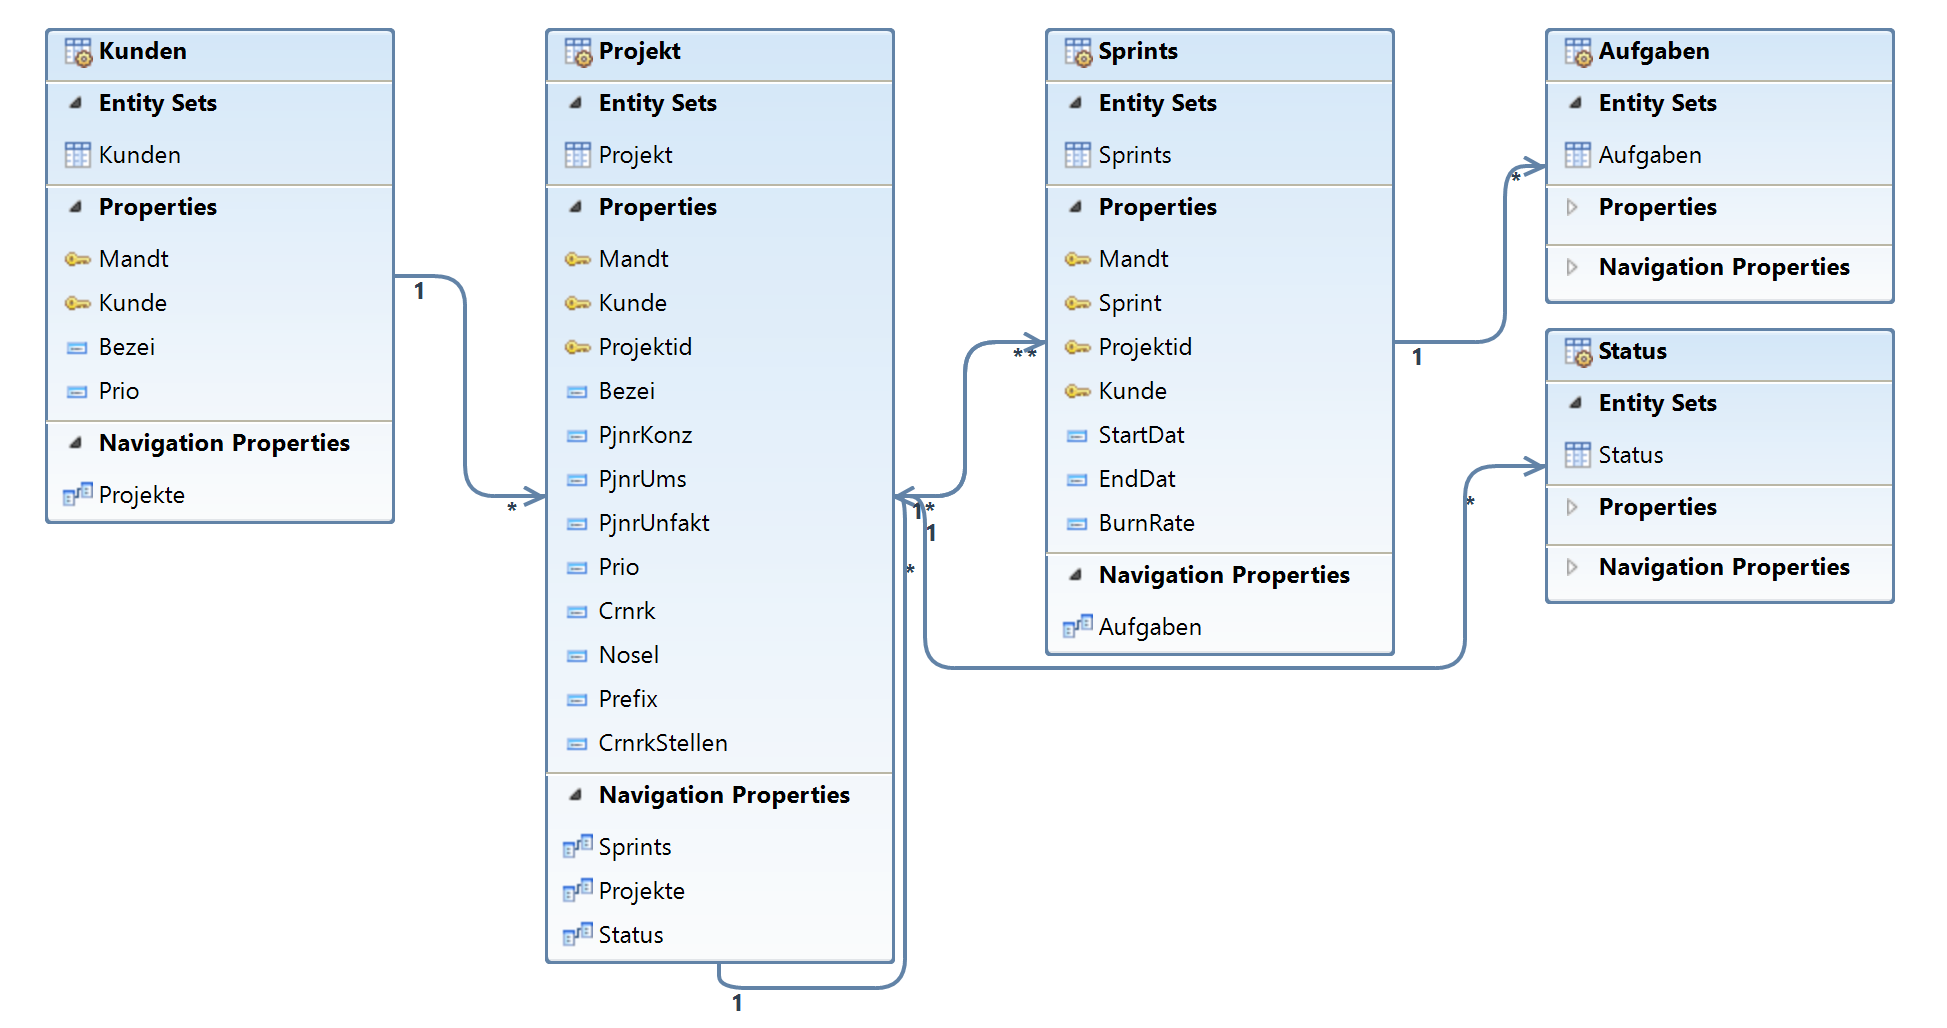
\includegraphics[width=1.25\textwidth]{odata-modeler} 
	\caption[OData Modeler]{OData Modeler.}
	\label{fig:OData-Modeler}
\end{figure}

\subsubsection{SAP Gateway Service Builder}
Das zentrale Werkzeug zur Erstellung von OData-Services ist der SAP Gateway Service Builder (Transaktion \emph{SEGW}). Der Service Builder enthält alle Funktionalitäten, die für die Serviceentwicklung benötigt werden \cite[S.\ 187-189]{BoennenDreesFischerHeinzStrothmann2014}. 


\subsubsection{Gateway-Client}
\label{sec:gateway-client}
Zum Testen des OData-Services wird der sogenannte Gateway-Client (Transaktion \emph{/IWFND/GW\_CLIENT}) verwendet. Mit ihm lassen sich alle Funktionalitäten des zuvor erstellten OData-Services testen. Testfälle lassen sich definieren und in Testgruppen zusammenzufassen, um sie später erneut auszuführen \cite[S.\ 190-192]{BoennenDreesFischerHeinzStrothmann2014}.


\subsubsection{Fehlerprotokoll}
Zur Fehlerbehandlung gibt es das Fehlerprotokoll unter der Transaktion \emph{/IWFND/ERROR\_LOG}. Hier laufen alle Fehler auf, die beim Aufruf von Gateway-Services auftreten. Bei Bedarf ist es dank Integration des Gateway Clients möglich, eine fehlerhafte Abfrage erneut auszuführen \cite[S.\ 192-193]{BoennenDreesFischerHeinzStrothmann2014}.
%193 - Syslog und Anwendungsprotokoll?

\subsubsection{Services aktivieren und verwalten}
In der Transaktion \emph{/IWFND/MAINT\_SERVICE} werden neue Services registriert und aktiviert. Ausgewählte Services lassen sich im Browser oder Gateway-Client testen und das dazugehörige Fehlerprotokoll wird, wenn nötig, geöffnet \cite[S.\ 571-573]{BoennenDreesFischerHeinzStrothmann2014}.


\subsection{Funktionsbausteine}
Für den Zugriff auf Daten aus dem SAP-Backend werden in der zentralen Aufgabenverwaltung derzeit Funktionsbausteine verwendet. Diese werden remotefähig gemacht, um über die \ac{RFC}-Schnittstelle aufrufbar zu sein. Für die Abfrage der Daten werden die \ac{RFC}-Funktionsbausteine vom OData-Service mit entsprechenden Parametern aufgerufen. Die RFC-Funktionsbausteine kommen dann beim Lesen der Kunden-, Projekt-, Sprint-  und Aufgabendaten sowie der möglichen Aufgabenstatus der einzelnen Projekte zum Einsatz. 

\begin{listing}[H]
	\inputminted{abap}{src/fubaprojekte.abap}
	\caption{Z\_SCRUMUI5\_READ\_PROJEKTE}
	\label{lst:Quellcode-ReadProjekte}
\end{listing}

\subsubsection{Entwicklung}
In allen Funktionsbausteinen werden Importparameter definiert, die vom OData-Service übergeben werden können. Dieses sind in der Regel die Primärschlüssel der Datenbanktabellen, auf die durch einen Funktionsbaustein zugegriffen wird, um eindeutige Datensätze auslesen zu können. Zusätzlich wird ein Parameter zur Filterung nach Teil-Strings definiert. Die ausgelesenen Daten werden über eine Tabelle, mit der Struktur der ursprünglichen Datenbanktabelle, zurückgegeben.

Im Listing \ref{lst:Quellcode-ReadProjekte} wird der Funktionsbaustein zum Auslesen der Projektdaten dargestellt. Es gibt drei mögliche Szenarien zum Aufruf des Bausteins mit den jeweils nötigen Übergabeparametern:

\begin{enumerate}
	\item Alle Projekte eines Kunden (KundenID)
	\item Ein bestimmtes Projekt des Kunden (KundenID, ProjektID)
	\item Projekte des Kunden die Teil-String enthalten (KundenID, ProjektID)
\end{enumerate}
In den ersten beiden Szenarien werden einfache Select-Statements auf die Datenbanktabellen ausgeführt um auf die Daten zuzugreifen. Da mit dem SQL Like Operator im Open SQL die Nichtbeachtung von Groß- und Kleinschreibung nicht möglich ist, wird im letzten Szenario, nach dem Select-Statement, durch alle zurückgegebenen Datensätze gelaufen und überprüft ob der übergebene Teil-String in der Bezeichnung des Projektes vorhanden ist. Hierbei ist es dann egal, ob die Groß- und Kleinschreibung des Datenbankeintrages identisch mit der des Teil-Strings ist.


\subsubsection{Testen}
Zum Testen von neuen Funktionsbausteinen gibt es in der ABAP Workbench die Funktion den jeweiligen Funktionsbaustein auszuführen und zu testen. Dazu wählt man in der Drucktastenleiste \textit{Testen/Ausführen (F8)}. Man gelangt auf das Bild \textit{Funktionsbaustein testen: Eingabebild}. Hier werden alle Import-Parameter des Funktionsbausteins angezeigt. Nach Eingabe der Parameter kann der Funktionsbaustein mit \textit{Ausführen (F8)} gestartet werden. Der Funktionsbaustein wird mit den eingetragenen Importparametern ausgeführt und vorhandene Exportparameter oder Tabellen werden nach Ausführung angezeigt. 


\begin{figure}[h]
	\centering
	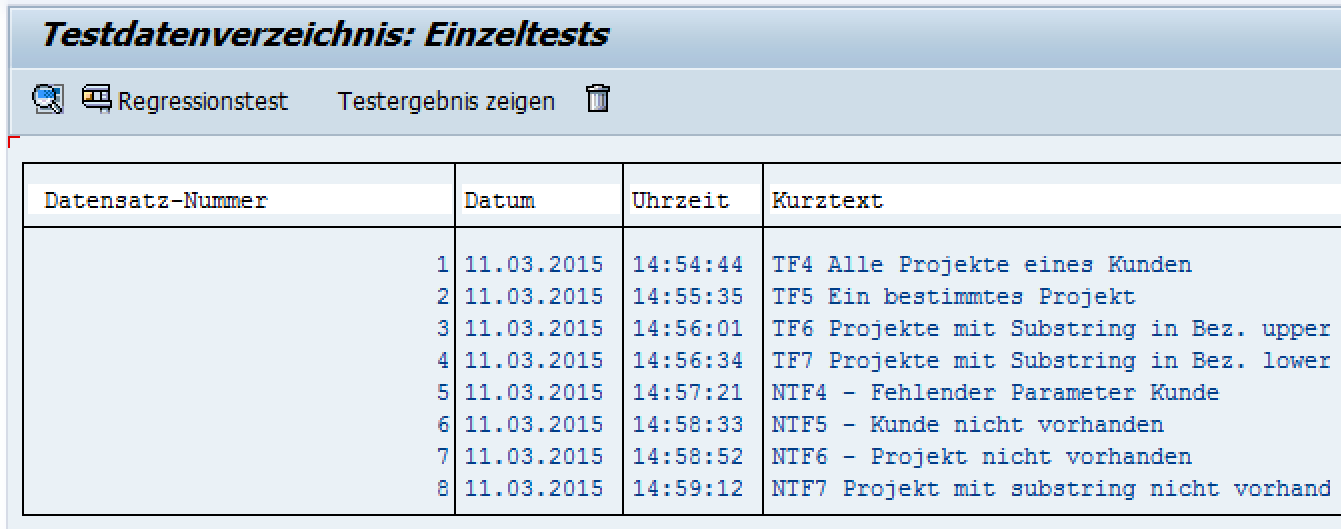
\includegraphics[width=.95\textwidth]{Testdatenverzeichnis} 
	\caption[Funktionsbaustein -- Testdatenverzeichnis]{Funktionsbaustein -- Testdatenverzeichnis.}
	\label{fig:Testdatenverzeichnis}
\end{figure}

\begin{figure}[h]
	\centering
	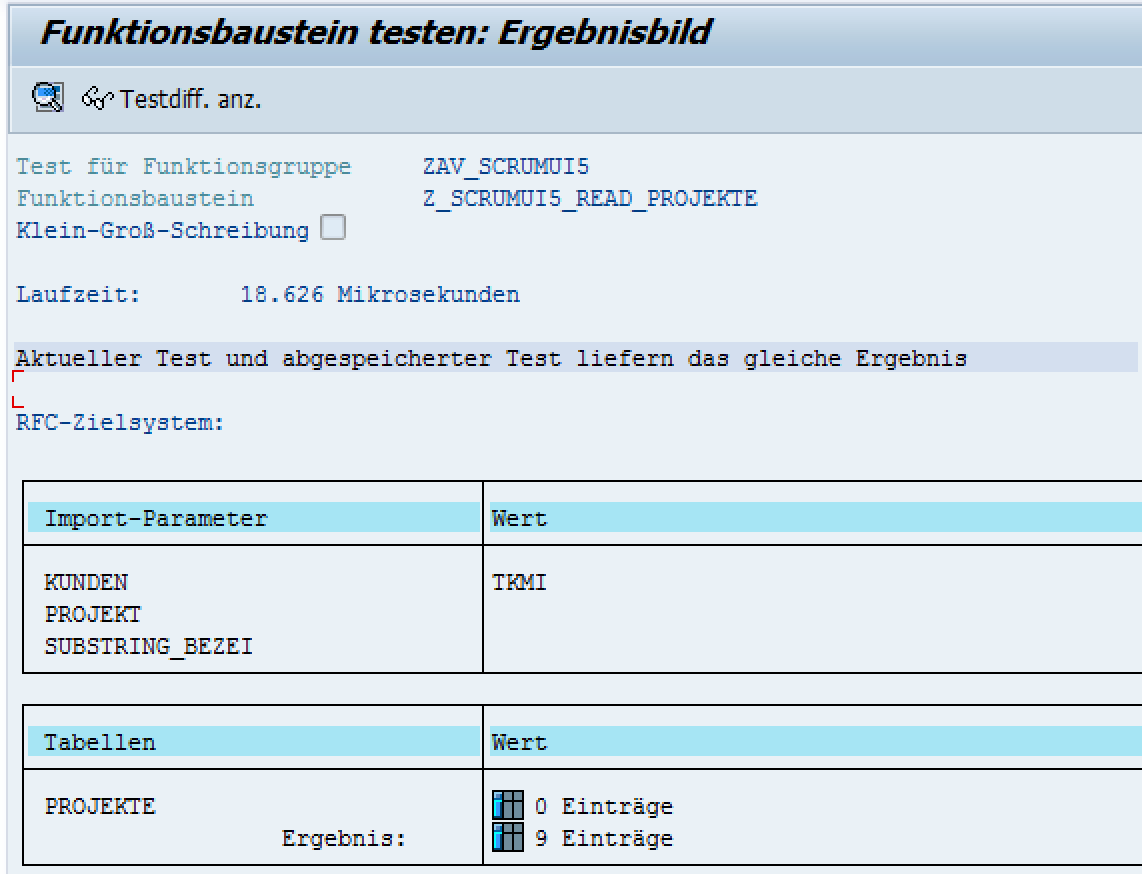
\includegraphics[width=.95\textwidth]{Regressionstest} 
	\caption[Funktionsbaustein -- Regressionstest]{Funktionsbaustein -- Regressionstest.}
	\label{fig:Regressionstest}
\end{figure}

Es ist möglich Testfälle im Testdatenverzeichnis zu speichern. Das Testdatenverzeichnis erreicht man über den ersten Eingabebildschirm. Alle gespeicherten Testfälle werden mit Erstelldatum und Kurztext wie in \autoref{fig:Testdatenverzeichnis} angezeigt und lassen sich hierüber erneut aufrufen. Bei Ausführung eines  Regressionstest wird im Ergebnis angezeigt ob sich das Ergebnis seit dem Speichern des Testes verändert hat, siehe \autoref{fig:Regressionstest}. Falls eine Differenz zum gespeichertem Ergebnis vorhanden ist, lässt sich diese anzeigen.\\ 



\subsection{OData-Service}
Für die Erstellung eines OData-Services im SAP Gateway gibt es generell unterschiedliche Wege: Zum einen gibt es die Serviceentwicklung mit \ac{ABAP}, welches flexiblere und effizientere Services ermöglicht. Diese erfordert allerdings spezielles \ac{ABAP}-Know-how. 

Alternativen dazu sind die Servicegenerierung durch den \ac{RFC}/\ac{BOR}-Generator, die Redefinition oder die Model Composition von bereits vorhandenen Gateway-Services. Die Servicegenerierung führt zu schnelleren Ergebnissen, ist durch eingeschränkte Rechte allerdings oft nicht weiter anpassbar.

Im Normalfall rechtfertigen die Vorteile durch die klassische ABAP-Service-Entwicklung den höheren Aufwand. Die Möglichkeit der Servicegenerierung wird interessant, sobald es geeignete Datenquellen für die automatische Generierung gibt \cite[S.\ 181]{BoennenDreesFischerHeinzStrothmann2014}.

Generell wird ein inkrementeller Serviceerstellungsprozess empfohlen, in dem der Service \bzw Teile davon direkt ausgeführt und getestet werden. Danach kann der Service so lange verändert werden, bis schließlich alle Anforderungen erfüllt werden \cite[S.\ 184]{BoennenDreesFischerHeinzStrothmann2014}.


\subsubsection{Entwicklung}
Die Entwicklung eines Gateway-Services lässt sich in drei Phasen einteilen:

\begin{quote}
	\begin{enumerate}
		\item Definition des Datenmodells
		\item Serviceimplementierung
		\item Serviceverwaltung
	\end{enumerate}
\end{quote}
%Definition des Datenmodells mit dem OData Modeler auf Basis der vorhandenen Struktur?
Zur \textit{Definition des Datenmodells} im SAP Gateway Service Builder gibt es unterschiedliche Varianten. 
Dazu zählen unter anderem die manuelle Deklaration des Datenmodells im Service Builder. Hierbei werden die Entitätstypen, Assoziationen und Assoziationsmengen manuell angelegt.

Alternativ kann ein bereits vorhandenes Datenmodell importiert werden, welches \zB mit dem OData Modeler erstellt wurde. Falls eine bereits vorhandene Datenstruktur aus einem SAP-System genutzt werden soll, können die Entitätstypen über einen DDIC-Import oder über den Import von \ac{RFC}/\ac{BOR}-Schnittstellen generiert werden \cite[S.\ 194-195]{BoennenDreesFischerHeinzStrothmann2014}.

\begin{figure}[h]
	\centering
	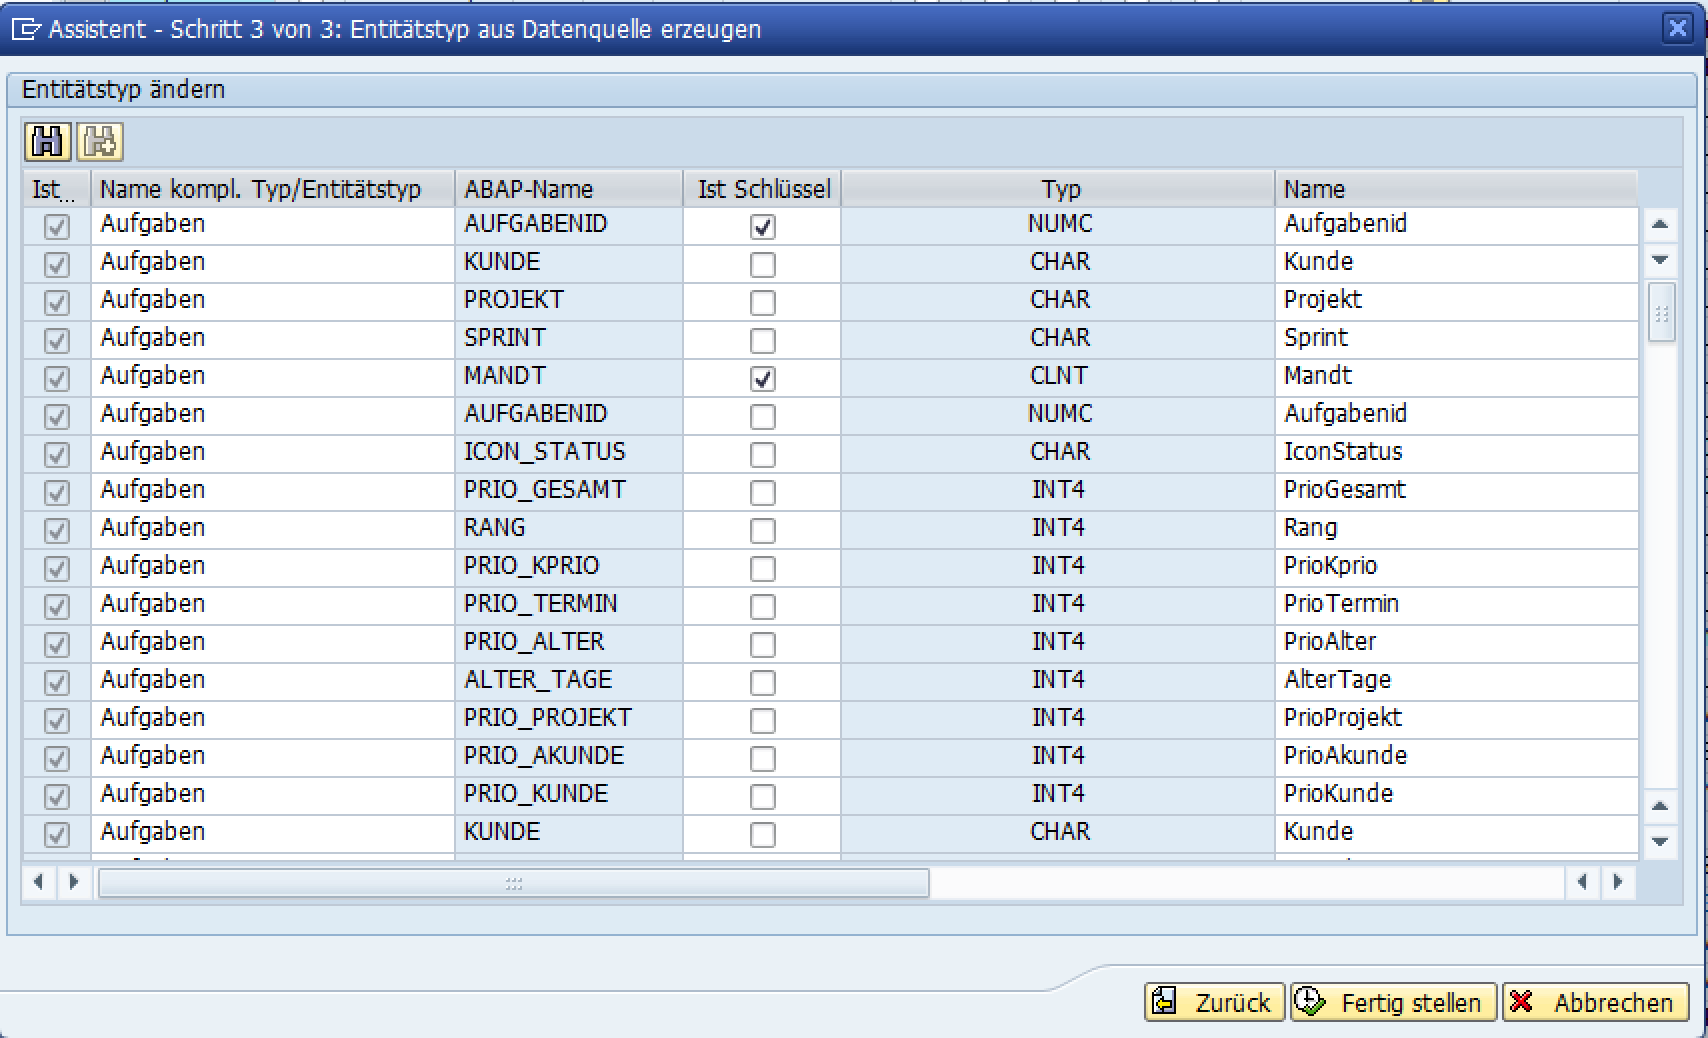
\includegraphics[width=.95\textwidth]{ImportRFC} 
	\caption[Import-RFC-Funktionsbaustein]{Import-RFC-Funktionsbaustein \cite[S.\ 45]{BoennenDreesFischerHeinzStrothmann2014}.}
	\label{fig:ImportRFC}
\end{figure}

In unserem Fall kommt der Import über RFC-Funktionsbausteine wie in \autoref{fig:ImportRFC} zum Einsatz, da diese auch für den Zugriff auf Daten aus dem SAP-Backend genutzt werden. Während des Imports des RFC-Funktionsbausteins müssen die Primärschlüssel der Entitätstypen festgelegt werden.

Unter den Eigenschaften der Entitätstypen lassen sich die einzelnen Attribute der Entitätstypen anzeigen und deren Eigenschaften ändern. So wird etwa definiert, ob ein bestimmtes Attribut sortier- oder filterbar ist. Diese Eigenschaften werden im Service-Metadatendokument hinterlegt. Diese haben allerdings nur einen informativen Charakter: Es erfolgt keine weitere Überprüfung durch das Gateway-Framework. So können Attribute sortiert werden, für die keine Sortier-Eigenschaft gesetzt wurde. 


Als nächstes müssen die Entitätsmengen definiert werden, die im Regelfall in einer 1:1-Beziehung zu den Entitätstypen stehen. Der spätere Zugriff über den OData-Service läuft immer über die Entitätsmengen und nicht über die Entitätstypen. Auch hier gibt es einige Attribute zu pflegen, \zB, ob ein Eintrag eines Entitätstypen angelegt, aktualisiert oder gelöscht werden darf, oder ein Filter für die Abfrage der Entitätsmenge zwingend erforderlich ist. Wie auch die Annotationen der Entitätstypen sind auch diese nicht zwingend bindend und erforderlich, sollten jedoch passend zum tatsächlichen Funktionsumfang des OData-Services gepflegt werden. So ist es für Service-Konsumenten einfacher herauszufinden, welchen Funktionsumfang der OData-Service unterstützt \cite[S.\ 237-240]{BoennenDreesFischerHeinzStrothmann2014}.


Anschließend wird der Service im SAP-System registriert. Hier werden die Laufzeitobjekte, die für den Gateway-Service benötigt werden, generiert \cite[S.\ 198]{BoennenDreesFischerHeinzStrothmann2014}.
Danach geht es an die \textit{Serviceimplementierung}. Hier gibt es die Auswahl zwischen der Implementierung durch ABAP-Programmierung  oder das Mappen von \ac{RFC}/\ac{BOR}-Schnittstellen \cite[S.\ 201-202]{BoennenDreesFischerHeinzStrothmann2014}.

\piccaption[RFC-Mapping]{RFC-Mapping\label{fig:MappingRFC}.}
\parpic{
	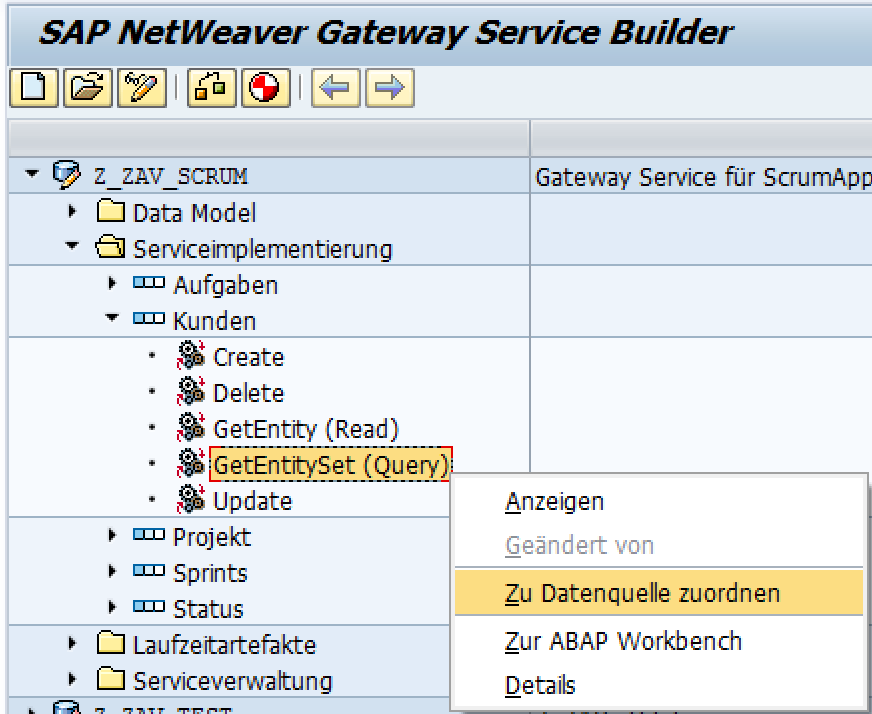
\includegraphics[width=.5\textwidth]{MappingRFC}
}

Um die Attribute einer En\-ti\-täts\-men\-ge mit einem RFC-Funk\-tions\-bau\-stein zu mappen, wählt man \emph{Zu Da\-ten\-quel\-le zuordnen} für den gewünschten Vorgang einer En\-ti\-täts\-men\-ge, hier: GetEntitySet der En\-ti\-täts\-men\-ge Kunden, siehe \autoref{fig:MappingRFC}.

Nach Angabe des Funk\-tions\-bau\-steins können die Attribute der Quelle zugeordnet werden. 

Dies funktioniert manuell oder über den Button \emph{Zuordnung vorschlagen} wie in \autoref{fig:MappingRFC2}. Zu diesem Zeitpunkt ist lediglich das Abrufen von Daten ohne zusätzliche Funktionen möglich. Um die Filterfunktionen des OData-Services nutzen zu können, müssen die Import-Parameter der Funktionsbausteine zugeordnet werden.

Dafür wird eine neue Zeile mit der Entitätsmenge des Importparameters hinzugefügt -- In diesem Fall \textit{Kunde}. Dieser wird dem Import-Parameter aus der Datenquelle zugeordnet. Jetzt kann nach bestimmten Kunden gefiltert werden.
So lassen sich Services mit Grundfunktionen relativ einfach durch die Servicegenerierung erstellen. Sobald Funktionen wie das Filtern nach Teil-Strings benötigt werden, ist eine Zusatzimplementierung durch ABAP-Programmierung notwendig.



\begin{figure}[h]
	\centering
	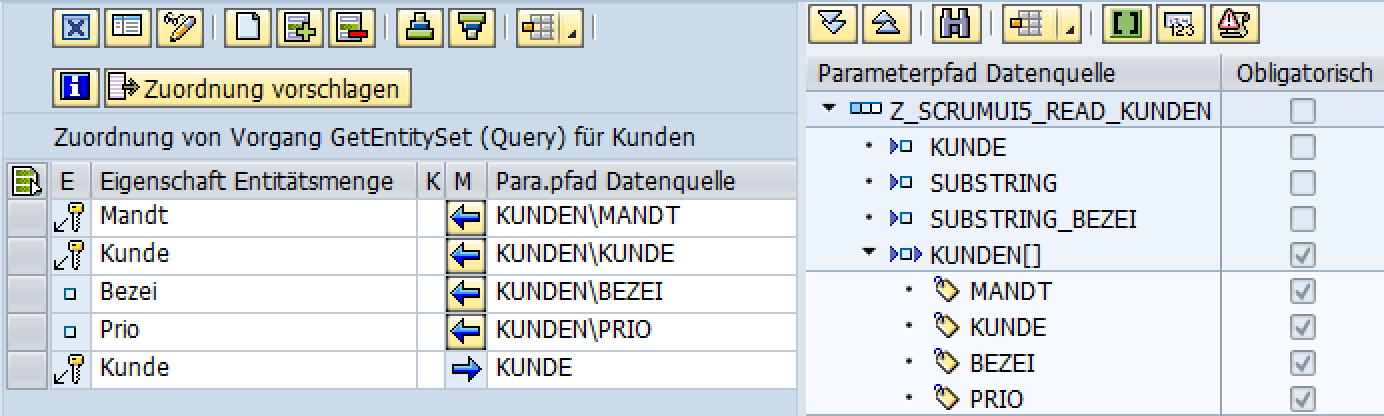
\includegraphics[width=.95\textwidth]{MappingRFC2} 
	\caption[RFC-Mapping -- Zuordnung der Attribute]{RFC-Mapping -- Zuordnung der Attribute.}
	\label{fig:MappingRFC2}
\end{figure}

Falls der Service durch ABAP-Programmierung erstellt werden soll, müssen die Methoden für den Vorgang in der ABAP-Workbench redefiniert werden. Die bei der Servicegenerierung automatisch erstellte Methode wird hier selbst implementiert. Alle Parameter, die vom OData-Service an das Gateway gesendet werden, müssen berücksichtigt und die entsprechenden Funktionen implementiert werden.

In \autoref{tab:ODataQueryOptions} gibt es eine kurze Übersicht, der vom SAP Gateway unterstützen OData-Query-Optionen, wovon einige eine zusätzliche Implementierung benötigen.

\begin{table}[h]
	\centering
	\begin{tabular}{cc}
		\toprule OData-Query-Optionen & Zusätzliche Implementierung notwendig \\ 
		\midrule \$select & Nein\\
		\$count & Nein\\
		\$expand & Nein\\
		\$format & Nein\\
		Read \$links & Nein\\
		\$value & Nein\\
		\$orderby & Ja\\
		\$top & Ja\\
		\$skip & Ja\\
		\$filter & Ja\\
		\$inlinecount & Ja\\
		\$skiptoken & Ja\\
		\bottomrule 
	\end{tabular} 
	\caption{Unterstützte OData-Query-Optionen im SAP Gateway aus \cite{SAP2015_3}}
	\label{tab:ODataQueryOptions}
\end{table} 



\begin{listing}[H]
	\inputminted{abap}{src/kundengetentityset.abap}
	\caption{KUNDEN\_GET\_ENTITYSET}
	\label{lst:Quellcode}
\end{listing}

In Listing \ref{lst:Quellcode} wird, falls in der Abfrage angegeben, ein Teil-String der Kundenbezeichnung in einer Variablen gespeichert. Diese wird anschließend an den Funktionsbaustein übergeben. Je nach Abfrage werden alle Kunden oder nur Kunden mit Teil-String im Namen zurückgegeben. Zum Abschluss werden die zurück erhaltenen Daten in die Tabelle \emph{ET\_ENTITYSET} geschrieben und an den OData-Service übergeben.

Nach Implementierung des Services muss dieser noch über die \textit{Serviceverwaltung} beim Gateway-Server registriert und aktiviert werden. Anschließend kann der OData-Service getestet werden.
Sind voneinander abhängige Entitätstypen im Service vorhanden, werden die Relationen mit den entsprechenden Kardinalitäten zwischen den Entitätstypen in den Assoziationen wie in \autoref{fig:Assoziationen} definiert. Die zuvor erstellten Assoziationen werden anschließend den Entitätstypen als Navigationseigenschaften zugewiesen, siehe \autoref{fig:Navigationseigenschaften}.

\begin{figure}[h]
	\centering
	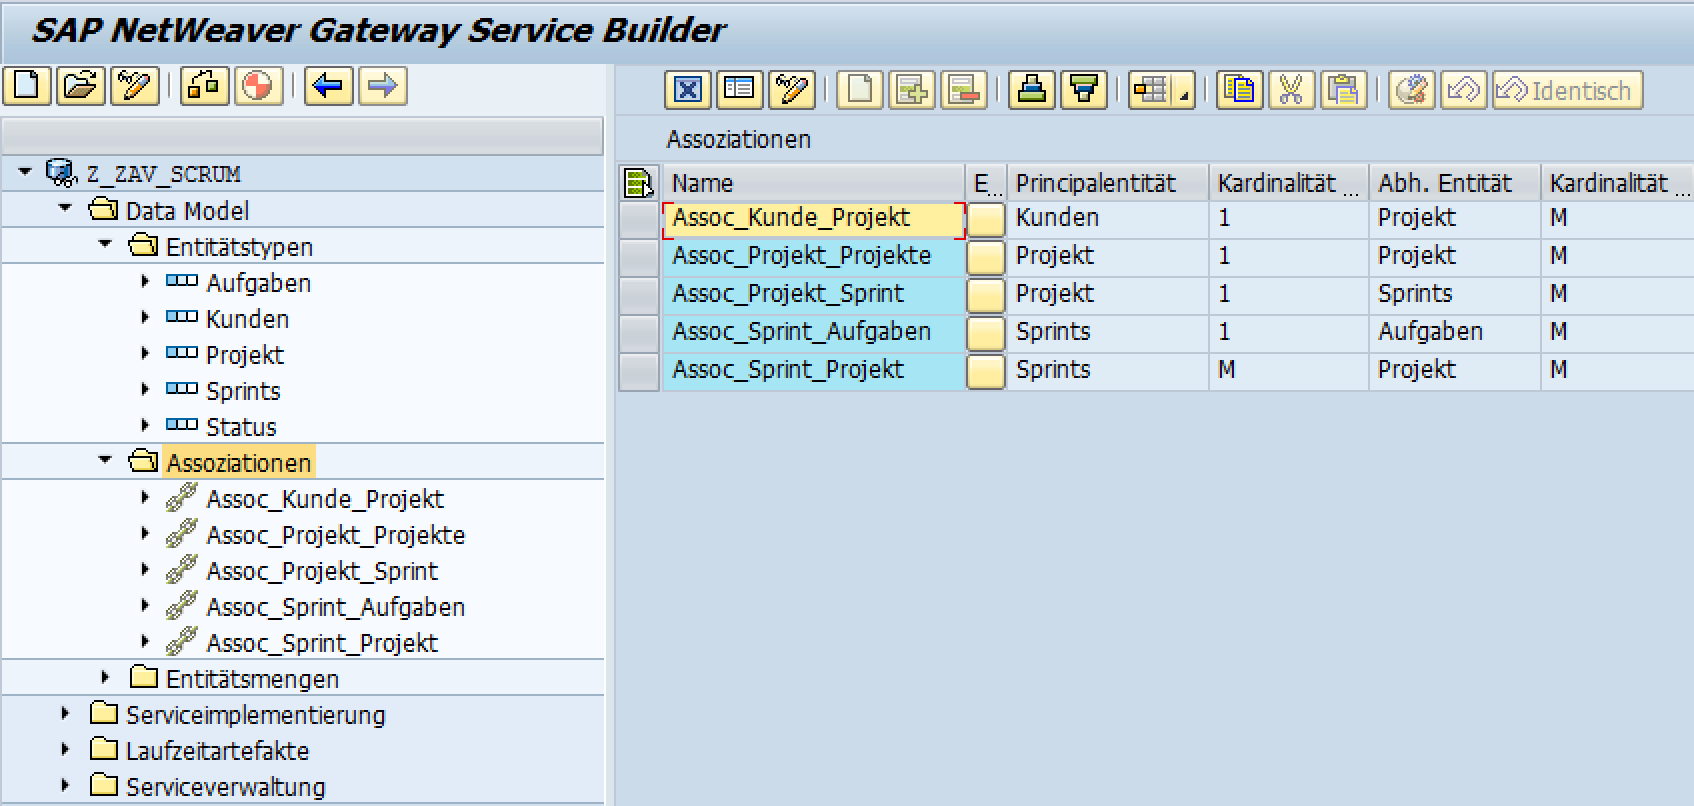
\includegraphics[width=.95\textwidth]{Assoziationen} 
	\caption[Entitätstypen -- Assoziationen]{Assoziationen zwischen den Entitätstypen.}
	\label{fig:Assoziationen}
\end{figure}


\begin{figure}[h]
	\centering
	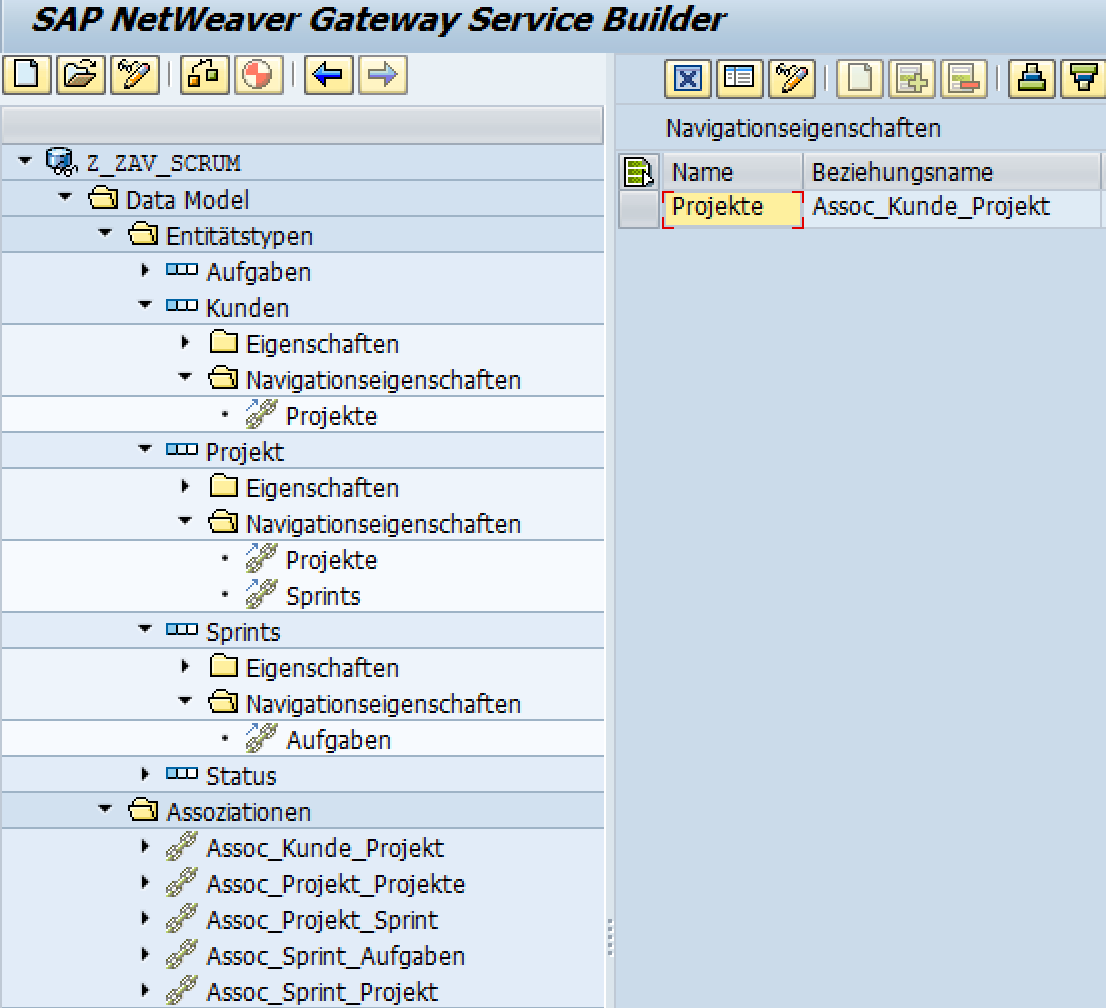
\includegraphics[width=.75\textwidth]{Navigationseigenschaften} 
	\caption[Entitätstypen -- Navigationseigenschaften]{Navigationseigenschaften zwischen den Entitätstypen.}
	\label{fig:Navigationseigenschaften}
\end{figure}


\subsubsection{Testen}

\begin{figure}
	\centering
	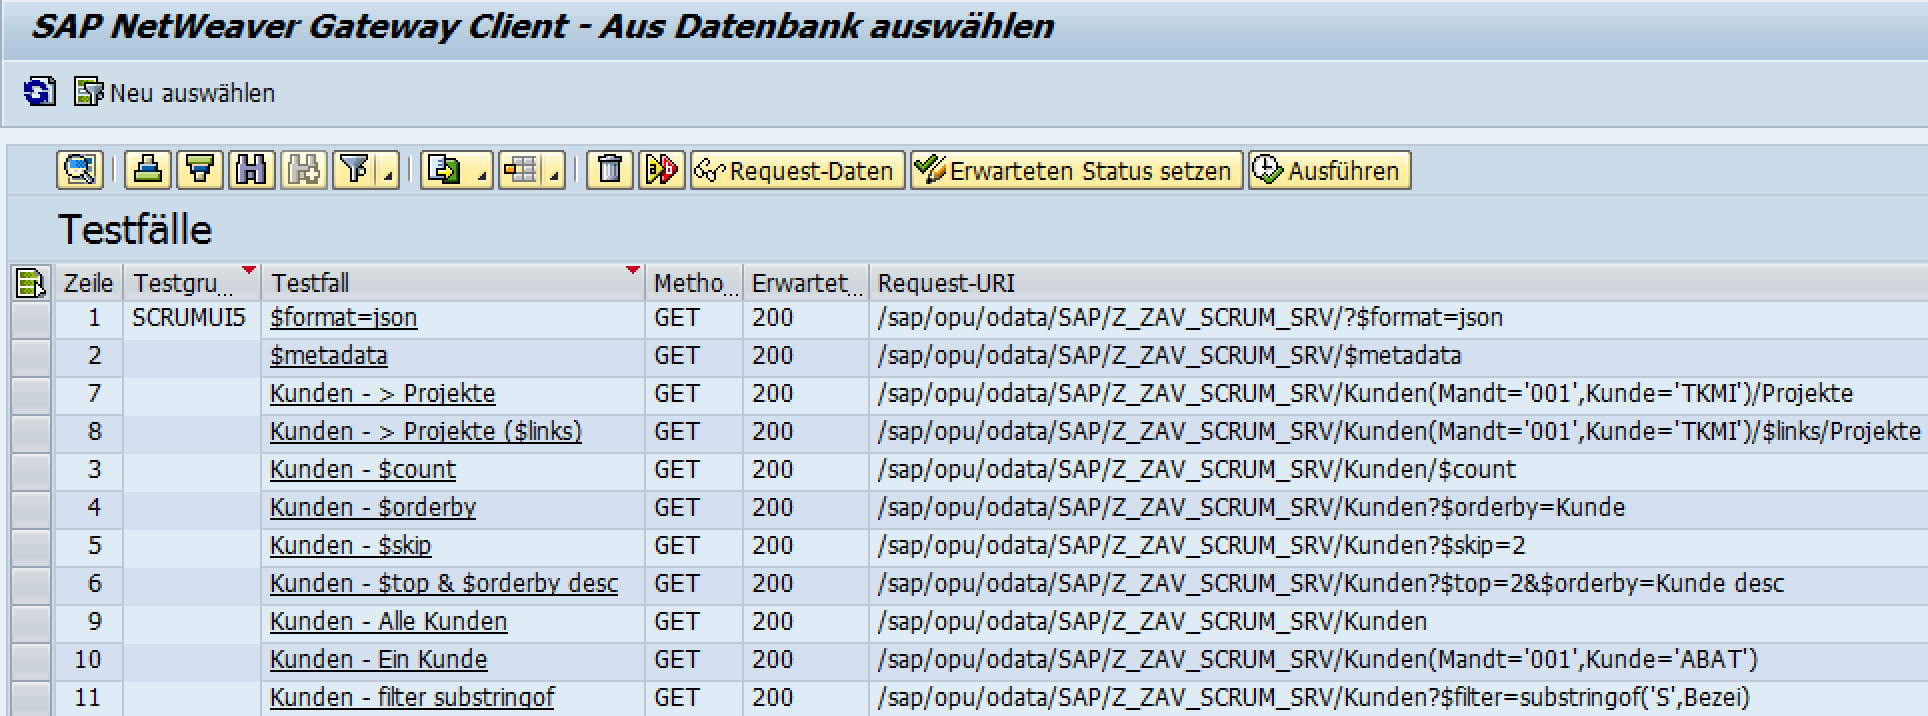
\includegraphics[width=.95\textwidth]{Testfalldatenbankodata} 
	\caption[OData-Testfalldatenbank]{OData-Testfalldatenbank.}
	\label{fig:Testfalldatenbankodata}
\end{figure}


\begin{figure}
	\centering
	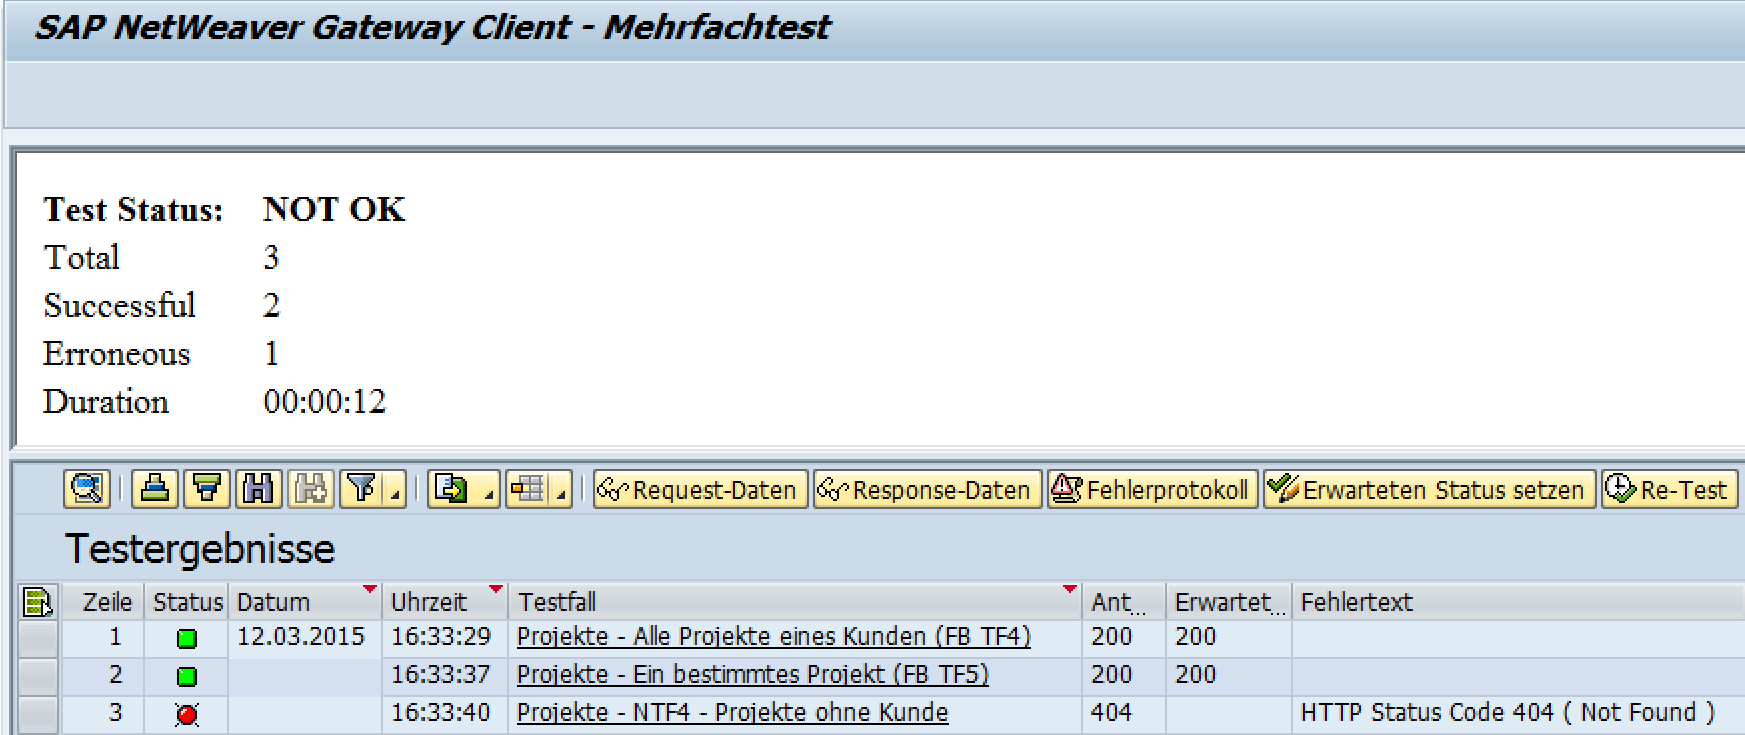
\includegraphics[width=.95\textwidth]{Mehrfachtest} 
	\caption[OData-Mehrfachtest]{OData-Mehrfachtest.}
	\label{fig:Mehrfachtest}
\end{figure}

Ist der OData-Service erstellt und registriert, geht es an das Testen mit dem SAP Gateway Client. Wie bereits in \autoref{sec:gateway-client} erwähnt, lassen sich die Testfälle für den OData-Service in Testgruppen speichern, und jederzeit wieder abspielen, siehe \autoref{fig:Testfalldatenbankodata}. Das Abspielen geschieht in einer sequenziellen Reihenfolge, um so komplexe Szenarien mit Erstellung, Update, Lesen und Löschen von Daten zu testen. Zu jedem abgesicherten Testfall lässt sich ein erwarteter HTTP-Statuscode definieren, wie in etwa der Code \textit{200} für den Status \textit{OK} oder \textit{4xx} für Client-Fehler \cite[S.\ 555-556]{BoennenDreesFischerHeinzStrothmann2014}.


Nach Ausführung der Testfälle gibt es eine Übersicht wie in \autoref{fig:Mehrfachtest}, inklusive erwartetem und tatsächlichem HTTP-Statuscode, sowie möglichem Fehlertext. Durch die Integration des Fehlerprotokoll lässt sich über die Auswahl eines fehlgeschlagenen Tests direkt in das Fehlerprotokoll wechseln, um die Fehlerursache zu ermitteln. 

Zusätzlich kann im Browser die Query-Option \textit{sap-ds-debug=true} genutzt werden, um Antworten des Services im Browser als HTML-Seite anzeigen zu lassen. Neben der Rückantwort gibt es zusätzliche Informationen wie \zB die Laufzeitanalyse der ABAP Methoden. Falls Fehler im Service auftreten, erscheint der Tab \textit{Stacktrace}, in dem die auftretende Exception angezeigt wird \cite[S.\ 555-556]{BoennenDreesFischerHeinzStrothmann2014}.


%\section{Ergebnisse}

\section{CI-Toolchain}
%Kurze Vorstellung aller Tools? 
%NodeJS
%Bower
%PhonegapBuild oder ans Ende hinter Jenkins?
%Karma
%Grunt
%Jenkins
%Zusammenfassung?
\autsubsection{Paketmanager}{Mattfeld}

Die Paketmanager sind existenzieller Bestandteil der \ac{CI}-Toolchain -- Das Prinzip \textit{Infrastructure as Code} ist nur mit ihrer Hilfe umzusetzen: Die Abhängigkeiten müssen nicht mehr in die Versionskontrolle eingecheckt werden, stattdessen werden die benötigten Versionen bei Bedarf extern nachgeladen.

\subsubsection{Node.js}
Node.js ist eine JavaScript-Laufzeitumgebung und für diverse Plattformen verfügbar. Basis ist die schnelle JavaScript-Engine Google V8, die um Techniken wie Nebenläufigkeit und nicht-blockierende I/O-Zugriffe erweitert wurde. Node.js kann eine große Zahl an gleichzeitigen Netzwerkverbindungen verwalten, ein zusätzlicher HTTP-Server ist nicht erforderlich. Ursprünglich sollte Node.js den einfachen Betrieb von Echtzeit-Webanwendungen ermöglichen.

Für dieses Projekt nutzen wir Node.js nicht als Server, sondern machen uns das stark gewachsene Ökosystem in Form des Node.js Package Managers \textit{npm} zu nutze. npm ist dabei zum einen ein lokales Tool zur Paketverwaltung, das direkt mit Node.js ausgeliefert wird, zum anderen gibt es ein zentrales Repository mit downloadbaren Paketen.

Diese Prinzip fördert eine hohe Modularisierung: JavaScript-typisch existieren viele kleine Tools, die eine bestimmte Aufgabe lösen, siehe \autoref{sec:tddjs}. Alle im Projekt genutzten Entwicklungs- und Testtools beziehen wir über npm.
Die Installation erfolgt nicht global, sondern lokal im Projektverzeichnis \textit{node\_modules}. Für verschiedene Projekte kann das gleiche Tool ohne Probleme in verschiedenen Versionen installiert werden. 

Formal ist auch unser UI5-Projekt selbst ein Node.js-Paket. Die Metadaten in der Datei \textit{package.json}, siehe Listing \ref{lst:package.json}, beschreiben es mit Namen und Version. Wir definieren zusätzlich alle Entwicklungsabhängigkeiten. Über den Befehl \textit{npm install} werden diese automatisch in der angegebenen Version installiert. Auch weitere, indirekte Abhängigkeiten werden aufgelöst. Ein neues Tool wird über \textit{npm install package -{}-save-dev} installiert und automatisch, als weitere Abhängigkeit für zukünftige Installationen, gespeichert.

Der Zusatz \textit{private} in der Konfiguration stellt sicher, dass wir das Paket nicht unabsichtlich über \textit{npm} veröffentlichen. Zusätzlich können private Repositories erstellt werden. So ist \zB eine firmeninterne, projektübergreifende Nutzung von Komponenten möglich.

Als Best Practice haben sich feste Versionen der Entwicklungsabhängigkeiten erwiesen. Im Gegensatz zu einem echten Node.js-Projekt sind sie bei uns nur ein Werkzeug und müssen keine breite Kompatibilität mit externen Abhängigkeiten eines veröffentlichten Pakets gewährleisten. Eine einmal funktionierende Konfiguration sollte beibehalten werden, um den Testaufwand der Infrastruktur gering zu halten.

\begin{listing}[H]
	\inputminted{json}{src/package.json}
	\caption{package.json (gekürzt)}
	\label{lst:package.json}
\end{listing}

\subsubsection{Bower}
Der zweite Paketmanager Bower ist nur für Frontend-Frameworks zuständig. In diesem Fall installiert er die UI5-Kernkomponenten \textit{sap.ui.core, sap.m} und das Standardtheme \textit{sap\_bluecrystal} im Projektordner unter \textit{bower\_\-components}. Sie sind zwar als Entwicklungsabhängigkeiten aufgeführt, wir nutzen sie aber gleichzeitig für das Release der App. Ein Grunt-Task kopiert die minified-Versionen in den Target-Ordner. Der Verwaltungs- und Testaufwand wird minimiert, weil für Entwicklung und Release die gleiche Version genutzt wird. Im Gegensatz zum offiziellen OpenUI5-Paket sind beim Bezug über Bower außerdem die Test-Frameworks QUnit und OPA5 enthalten.

Die automatische Paketinstallation wird über \textit{bower install} angestoßen. Auch die Paket-Verwaltung erfolgt synchron zu npm zentral über die Datei \textit{bower.json}, siehe Listing \ref{lst:bower.json}.
Im Unterschied zu npm unterstützt Bower keine geschachtelten Abhängigkeiten. Jedes Framework existiert nur einmal im Projekt -- Der Verzeichnisbaum hat nur eine Ebene. Bower arbeitet dadurch schneller als npm. 
Die einfache Struktur zwingt außerdem dazu, eine kompatible Framework-Kombination zu finden. Für den Endbenutzer führt dies zu schnelleren Ladezeiten, da nur jeweils eine Version heruntergeladen werden muss.

Mittelfristig wird Bower durch den mächtigeren npm abgelöst. Der Pflegeaufwand für zwei Paketmanager ist hoch. Viele Projekte haben dies erkannt, und bieten auch ihre Frontend-Frameworks per npm an. Bei OpenUI5 ist dies aber noch nicht der Fall.

\begin{listing}[H]
	\inputminted{json}{src/bower.json}
	\caption{bower.json (gekürzt)}
	\label{lst:bower.json}
\end{listing}

\autsubsection{Statische Analyse mit ESLint}{Mattfeld}
Da JavaScript nicht kompiliert wird, werden Syntax-Fehler erst während der Ausführung erkannt. Die statische Code-Analyse setzt schon vorher, während der Bearbeitung im Editor, an. Häufige Fehler oder sogenannte Anti-Patterns (nicht empfohlene Vorgehensweisen) sind global deklarierte oder nie genutzte Variablen. Außerdem lassen sich bestimmte Code-Styleguides durchsetzen.

ESLint ist ein Open-Source-Projekt auf Node.js-Basis. Die Installation erfolgt entsprechend per npm. ESLint bringt bereits ein vordefiniertes Regelset mit. Im Gegensatz zu JSLint oder JSHint ist dieses jedoch vollständig frei konfigurierbar. In der Datei \textit{.eslintrc} werden die vorhandenen Regeln als Warnung oder Fehler eingestuft -- oder ignoriert. Globale Variablen sind frei definiert oder umgebungsspezifisch als gültig deklariert, \zB im Node.js- oder jQuery-Kontext.

Wir übernehmen das Regelset aus OpenUI5. Zusätzlich nutzen wir das Plugin \textit{eslint-openui5}, das eine weitere UI5-spezifische Regel für Zeilenenden hinzufügt. Besonderheit: Weder das UI5-Framework, noch die Best-Practice-Beispiele sind mit den Regeln konform. \ZB das mittlerweile obligatorische \textit{'use strict';} fehlt. Das von SAP veröffentlichte Regelset ist eher Ziel, als aktueller Standard. Entsprechend unterziehen wir das Framework keiner statischen Prüfung. Unsere Eigenentwicklungen sind allerdings ESLint-konform, um zukünftige Kompatibilität zu gewährleisten.

\autsubsection{Testtreiber Karma}{Mattfeld}
\label{sec:karma}
Karma ist ein JavaScript-Testtreiber auf Node.js-Basis und aus dem Google-Projekt AngularJS hervorgegangen. Er ist das Verbindungsglied zwischen Test-Frameworks (Qunit, OPA5), CI-Tool (Grunt/Jenkins) und Browser (Desktop, Mobil, Headless, \dots). Die Architektur ist modular: Verbindungsfunktionen übernehmen Plugins, sogenannte Karma-Adapter.

Installiert wird karma per npm. Anschließend kann die Erstkonfiguration über \textit{karma init karma.conf.js} gestartet werden. Ein Assistent führt zu einer Minimalkonfiguration wie in Listing \ref{lst:karma.conf.js}. Wir benötigen die Test-Frameworks QUnit und OPA5. Außerdem speichern wir den Pfad zum OpenUI5-Framework und aktivieren dessen Mockserver. 

Beim Start per \textit{karma start}, bzw. über die IDE oder Jenkins/Grunt, stellt Karma bestimmte Dateien über seinen integrierten Server bereit. Die verschiedenen File-Anweisungen in der Konfiguration schließen OpenUI5, unsere App und die Tests ein (\textit{served}). Der Parameter \textit{watched} überwacht das angegebene Verzeichnis. Ändern sich App-Code oder Testdaten, wird ein erneuter Testlauf angestoßen. \textit{included} markiert die Verzeichnisse mit Testskripts.

Die weiteren Parameter aktivieren eine Code-Coverage-Protokollierung, automatische Regressionstests und den zu öffnenden Browser. Möglich wären hier statt Chrome auch diverse andere Desktop-Browser, mobile Geräte und ein Test ohne grafische Oberfläche per PhantomJS. \textit{singleRun} ist eine spezielle CI-Option: Karma beendet Server und Browser automatisch nach einem Testlauf.

\begin{listing}[H]
	\inputminted[tabsize=2]{js}{src/karma.conf.js}
	\caption{karma.conf.js -- Minimalkonfiguration}
	\label{lst:karma.conf.js}
\end{listing}

Speziell für unser UI5-Projekt benötigen wir den Adapter \textit{karma-openui5}\footnote{\url{https://github.com/SAP/karma-openui5}}. Er lädt OpenUI5 aus dem bereits angegebenen Verzeichnis. Zusätzlich werden wie in Listing \ref{lst:karma.openui5.conf.js} die weiteren Bibliotheken und Themes bereitgestellt. Die Konfiguration erfolgt analog zum UI5-Bootstrapping.

\begin{listing}[H]
	\inputminted[tabsize=2]{js}{src/karma.openui5.conf.js}
	\caption{karma.conf.js -- Ausschnitt OpenUI5}
	\label{lst:karma.openui5.conf.js}
\end{listing}

Der Mockserver wird wie in Listing \ref{lst:karma.mockserver.conf.js} konfiguriert. \textit{rootURI} entspricht der OData-Service-Adresse, die unsere App aufruft. Der Mockserver fängt entsprechende Aufrufe ab und stellt einen, anhand der \textit{metadata.xml} definierten, Service bereit. Diese kann per OData Modeler erstellt, oder von einem bereits verfügbaren Service exportiert werden.

Unter \textit{mockdataSettings} ist das Verzeichnis der Mock-Daten angegeben, also die Objekte, die der Server zurückliefert. In diesem Projekt sind das \zB \textit{Kunden.json} oder \textit{Projekt.json}, die wir aus dem laufenden Service exportiert haben. Alternativ erzeugt der Mockserver auch Zufallsdaten aus der Spezifikation.

\begin{listing}[H]
	\inputminted[tabsize=2]{js}{src/karma.mockserver.conf.js}
	\caption{karma.conf.js -- Ausschnitt Mockserver}
	\label{lst:karma.mockserver.conf.js}
\end{listing}

Zur Zeit (Stand: 12.03.2015) ist der Adapter karma-openui5 nicht ohne Modifikation in unserer Toolchain lauffähig. Um die Mockserver-Funktion zu nutzen, muss die Datei \textit{./node\_modules/karma-openui5/lib/mockserver.js} in Zeile 7 erweitert werden. Listing \ref{lst:mockserver.js} zeigt den aktuellen Workaround. Das Problem ist gemeldet und in Klärung.

\begin{listing}[H]
	\inputminted[tabsize=2]{js}{src/mockserver.js}
	\caption{mockserver.js Erweiterung}
	\label{lst:mockserver.js}
\end{listing}

\autsubsection{Hybrid-App per PhoneGap Build}{Azimi}
PhoneGap Build\footnote{\url{http://build.phonegap.com}} ist ein Cloud-Service von Adobe um mobile Web-An\-wen\-dun\-gen auf Basis des Open Source Toolkits Apache Cordova in der Cloud zu kompilieren. 

\begin{figure}[h]
\centering
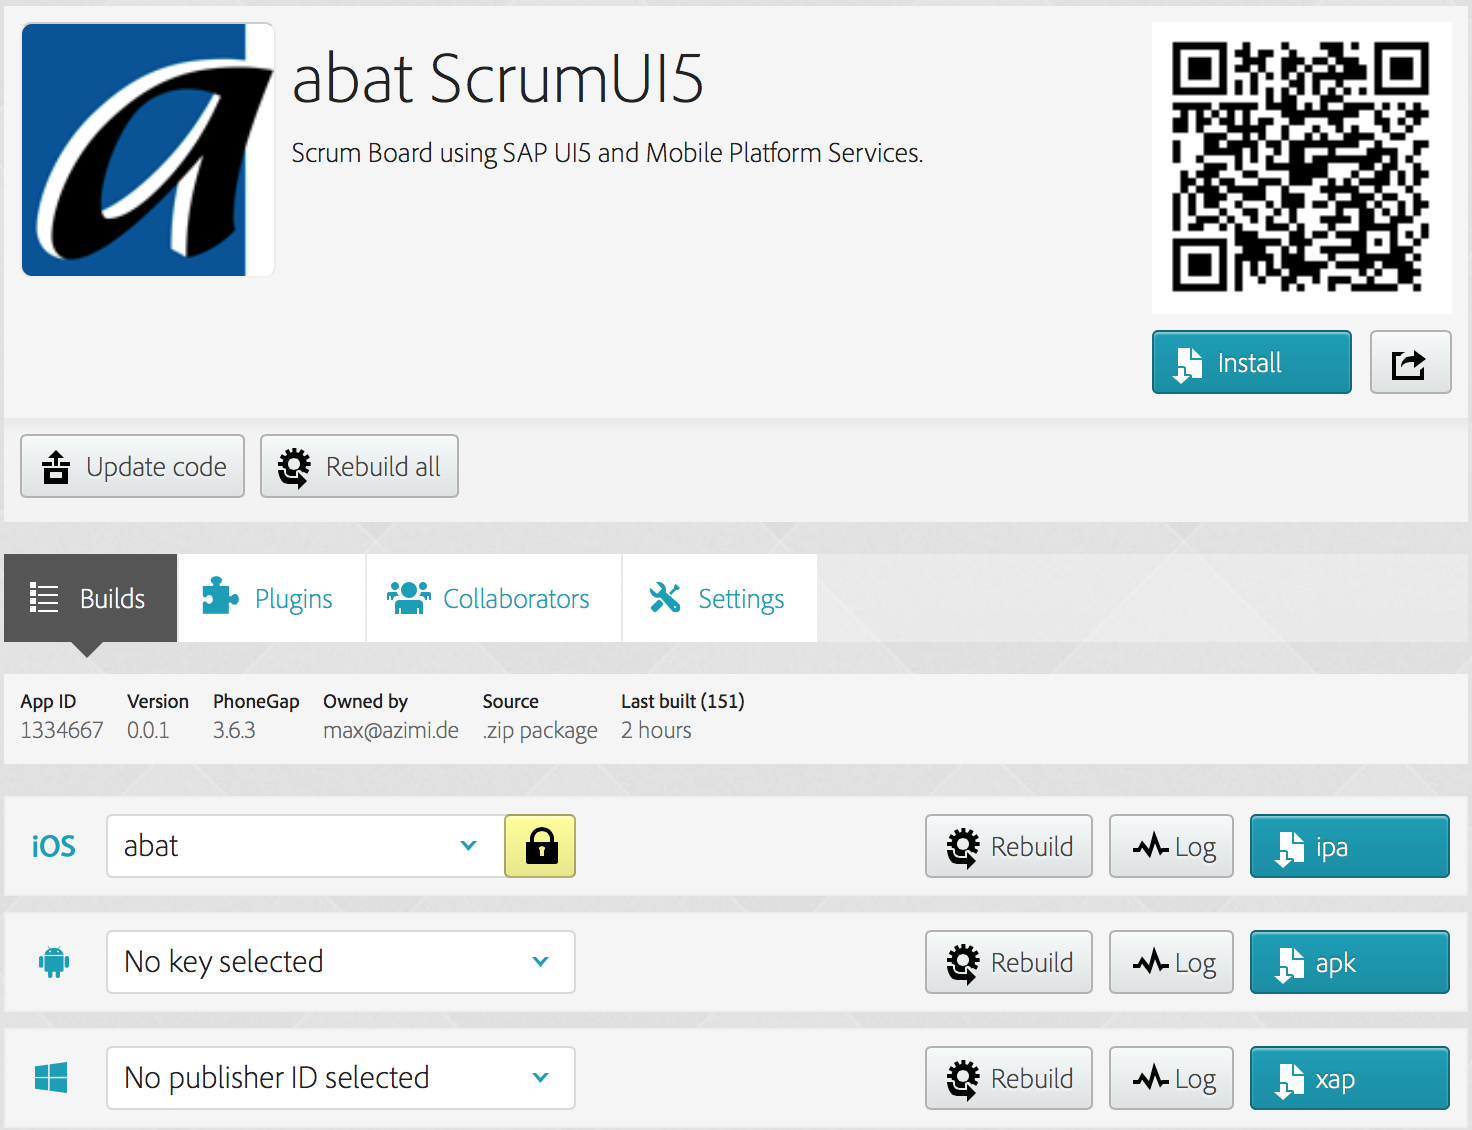
\includegraphics[width=.95\textwidth]{PhoneGapBuild}
\caption[PhoneGap-Build-Webinterface]{PhoneGap-Build-Webinterface.}
\label{fig:Phonegap}
\end{figure}

Die Konfiguration des PhoneGap Builds läuft über die Weboberfläche, die auf \autoref{fig:Phonegap} zu sehen ist. Der Quellcode der Web-Applikation kann als ZIP-Archiv gepackt und hochgeladen oder automatisch aus einem Git-Repository geladen werden. Anschließend wird die Anwendung für verschiedene Betriebssysteme direkt kompiliert und signiert. Für die Signierung der iOS-App müssen die  entsprechenden Entwicklerzertifikate hinterlegt werden.

Nach erfolgreichem Build der Anwendung können die Installationsdateien für die verschiedenen Plattformen heruntergeladen und für die weitere Verteilung genutzt werden. Zudem ist es möglich, die Anwendung über einen Link zu verteilen. Dieser installiert auf mobilen Geräten automatisch die App. 

Auf native Gerätefunktionen wird durch verschiedene Plugins zugegriffen, sodass Kamera oder GPS-Koordinaten auch für Web-Apps zugänglich sind. Durch das Kompilieren in der Cloud wird kein spezielles \ac{SDK} für die verschiedenen Plattformen wie iOS und Android benötigt. Es reicht eine Entwicklungsumgebung für Webanwendungen.

\autsubsection{JS Task Runner Grunt}{Azimi}
Um die Vielzahl an Werkzeugen für unseren automatischen Build aufzurufen, kommt der sogenannte JavaScript Task Runner Grunt\footnote{\url{http://gruntjs.com/}} zum Einsatz. Einzige Aufgabe ist die Abarbeitung der einzelnen Tasks, die in der Grunt-Konfiguration (siehe Listing \ref{lst:gruntfile}) definiert werden \cite[S.\ 59-61]{Wrobel2015}. Die eigentlichen Funktionalitäten sind in diverse Grunt-Plugins ausgelagert, die wir im Folgenden erläutern.

\begin{listing}
	\inputminted{javascript}{src/gruntfile-short.js}
	\caption{Auszug Gruntfile.js}
	\label{lst:gruntfile}
\end{listing}

\subsubsection{grunt-contrib-uglify}
Dies ist ein Grunt-Plugin zum Ausführen des UglifyJS-Toolkits. Hiermit wird der JavaScript-Code komprimiert, Variablennamen werden, wenn möglich, verkürzt und vorhandene Kommentare gelöscht. Die minified-JavaScript-Files besitzen typischerweise nur noch 30--40\,\% der Ursprungsgröße.
%  \cite{Uglify2015}

\subsubsection{grunt-eslint}
Überprüft den JavaScript-Code auf Einhaltung der vereinbarten Regeln zur statischen Code-Analyse per ESLint, einer Weiterentwicklung von JSHint. Hierfür stellt SAP im OpenUI5-Repository eine ESLint-Konfigurationsdatei zur Verfügung, die in eigenen Projekten verwendet werden kann \cite{SAP2015_2}.

\subsubsection{grunt-karma}
Dieses Plugin ermöglicht es, Karma während des Build-Prozesses aufzurufen. Über separate Karma-Tasks werden die Unit- und Akzeptanztests ausgeführt. \cite[S.\ 129-130]{Wrobel2015}.

\subsubsection{grunt-contrib-copy}
Verschiebt Dateien, \zB vom Source- in den Destination-Ordner.

\subsubsection{grunt-contrib-compress}
Komprimiert den Target-Ordner in einer ZIP-Datei, damit diese anschließend vom PhoneGap-Build-Plugin weiterverarbeitet wird.

\subsubsection{grunt-phonegap-build}
Lädt das in einer ZIP-Datei archivierte Projekt über ein \ac{API} zu PhoneGap Build. Anschließend löst es einen neuen Build aus und signiert die Installationsdateien.

\subsubsection{grunt-plato}
Neben der statischen Code-Analyse durch ESLint gibt es weitere Analysen des Quelltextes durch das plato-Plugin. Es stellt verschiedene Metriken zur Komplexität und Wartungsfreundlichkeit des Codes bereit.
%https://github.com/jsoverson/grunt-plato
%http://de.slideshare.net/JarrodOverson/complexity-28214103
%HIER MEHR SCHREIBEN!
\SuperPar
\SuperPar
\autsubsection{Jenkins}{Azimi}
Als Continuous-Integration-Server wird Jenkins\footnote{\url{https://jenkins-ci.org/}} eingesetzt. Für die Implementierung verschiedener Werkzeuge im Continuous-Integration-Prozess werden zusätzliche Plugins wie folgt verwendet:

\begin{figure}[h]
\centering
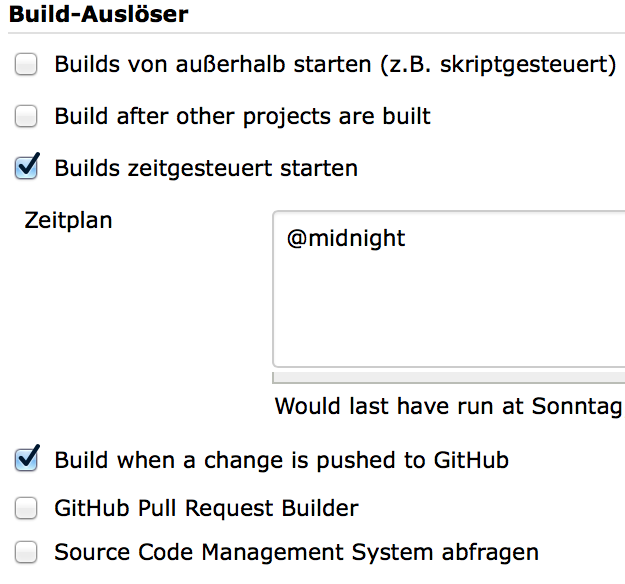
\includegraphics[width=.50\textwidth]{Github2-JenkinsConfig}
\caption[Build-Auslöser]{Build-Auslöser.}
\label{fig:Github2}
\end{figure}

\subsubsection{GitHub-Plugin}Zur Versionsverwaltung der Projektdaten wird GitHub verwendet. Das Plugin stößt den Build-Prozess bei Code-Änderungen im Repository automatisch an. Ebenfalls möglich ist eine zeitgesteuerte Ausführung oder ein manueller Start wie in \autoref{fig:Github2}. So ist gewährleistet, dass der Build inkl. Tests mit der aktuellen Version des Codes durchgeführt wird.

\subsubsection{Einbindung Paketmanager und Grunt}
Die Einbindung von Node.js, Bower und Grunt in den Continious-Integration-Prozess funktioniert durch Kommandozeilenbefehle, siehe \autoref{fig:Kommandozeile}, welche von Jenkins ausgeführt werden.

\begin{figure}[h]
\centering
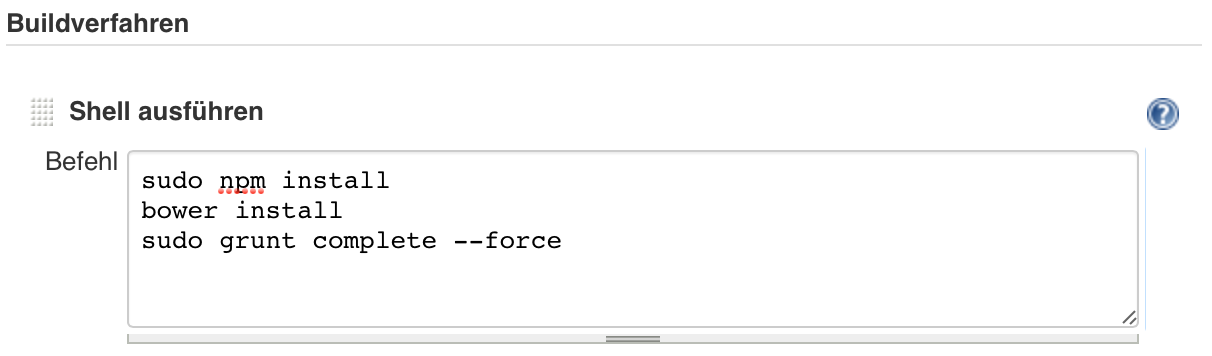
\includegraphics[width=.95\textwidth]{Kommandozeile}
\caption[Integration von Paketmanagern und Grunt]{Integration von Paketmanagern und Grunt.}
\label{fig:Kommandozeile}
\end{figure}


\subsubsection{Checkstyle}
Um die Ergebnisse des ESLint-Checks in Jenkins anzeigen zu können, wird das Jenkins-Checkstyle-Plugin genutzt. Dazu muss in der Jenkins-Projekt-Konfiguration der Pfad zu den Ergebnissen angegeben werden. Anschließend wird in der Projektübersicht ein Trend-Graph, wie in \autoref{fig:Checkstyle-Trendgraph} zu sehen ist, mit der Anzahl an Checkstyle-Warnungen erstellt. Zusätzlich lassen sich diese Warnungen je nach Verzeichnis, Datei oder Warnungs-Typ aufschlüsseln, vergleiche \autoref{fig:Checkstyle-Warnungen}.

\begin{figure}[h]
\centering
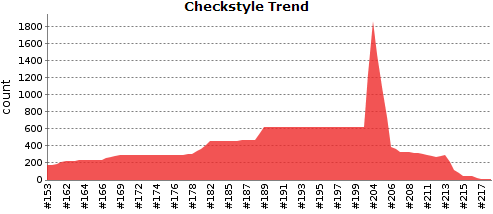
\includegraphics[width=.95\textwidth]{Checkstyle-Trendgraph} 
\caption[Checkstyle-Warnungen -- Trend-Graph]{Trend-Graph der Checkstyle-Warnungen.}
\label{fig:Checkstyle-Trendgraph}
\end{figure}

\begin{figure}[h]
\centering
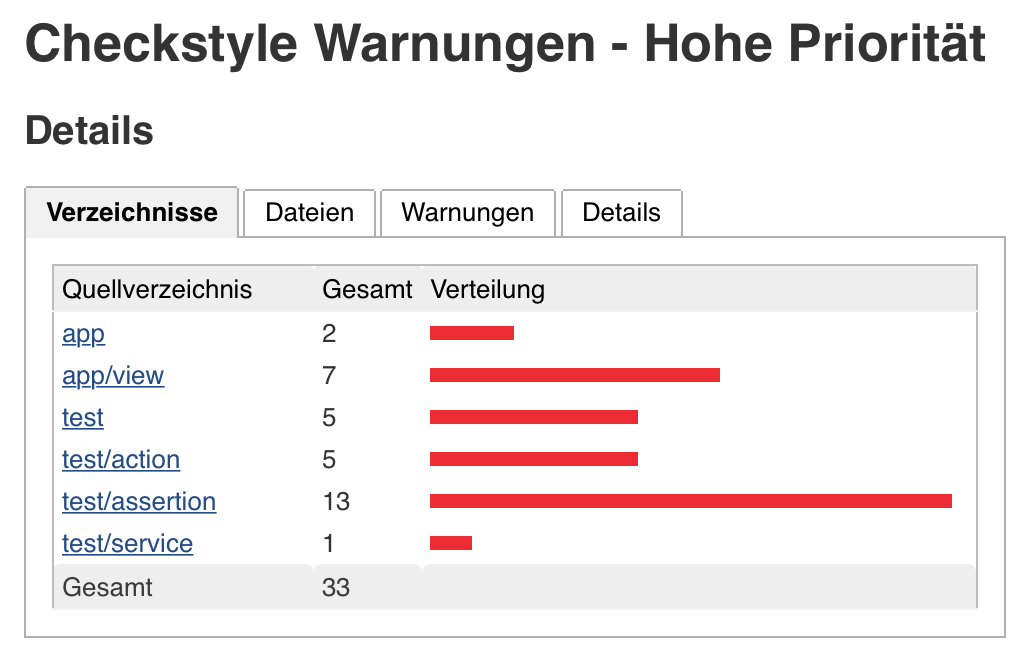
\includegraphics[width=.95\textwidth]{Checkstyle-Warnungen-high}
\caption[Checkstyle-Warnungen -- Hohe Priorität]{Checkstyle-Warnungen -- Hohe Priorität.}
\label{fig:Checkstyle-Warnungen}
\end{figure}

\subsubsection{Cobertura}
Zur Anzeige der Zeilenabdeckung aus den Akzeptanztests wird das Cobertura Plugin gebraucht. Das Plugin erzeugt einen Trend-Graphen, in dem die Zeilenabdeckung des Codes untergliedert in Pakete, Dateien, Klassen, Methoden, Zeilen und Verzweigung dargestellt wird, siehe \autoref{fig:CodeCoverage-Package}. Über den Graphen kann bis in die einzelnen Dateien und den dazugehörigen Quellcode navigiert werden. Welche Teile des Codes durch die ausgeführten Tests bisher abgedeckt bzw. eben nicht abgedeckt sind, wird hier nachvollziehbar, wie in \autoref{fig:CodeCoverage-Code} zu sehen ist.

\begin{figure}[h]
\centering
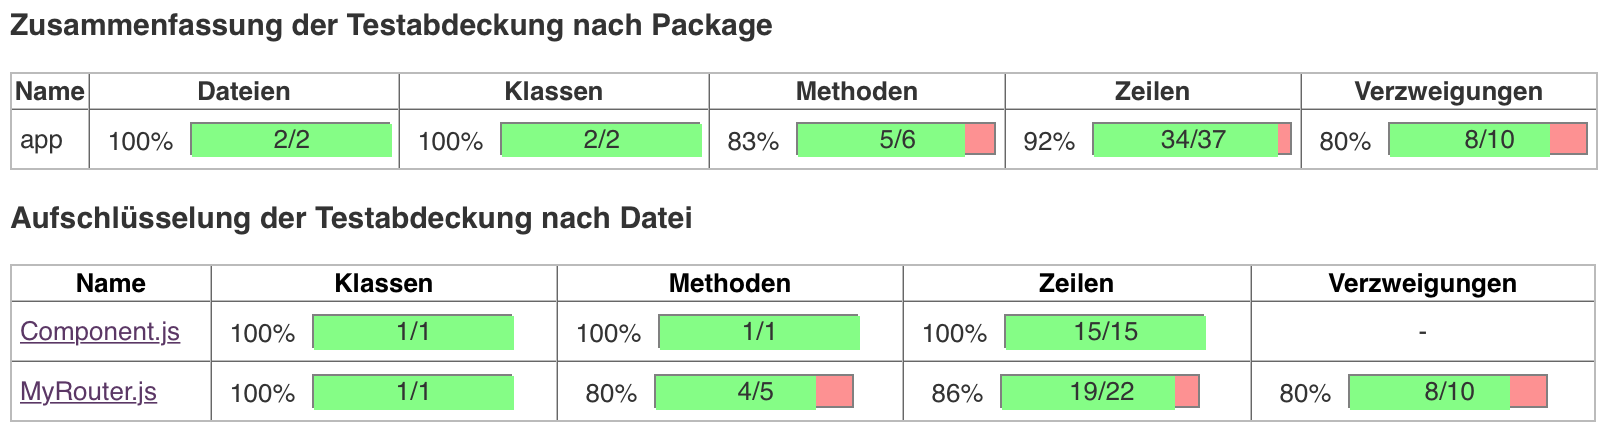
\includegraphics[width=1.25\textwidth]{CodeCoverage-Package}
\caption[Zeilenabdeckung im Paket \emph{app}]{Zeilenabdeckung im Paket \emph{app}.}
\label{fig:CodeCoverage-Package}
\end{figure}

\begin{figure}[h]
\centering
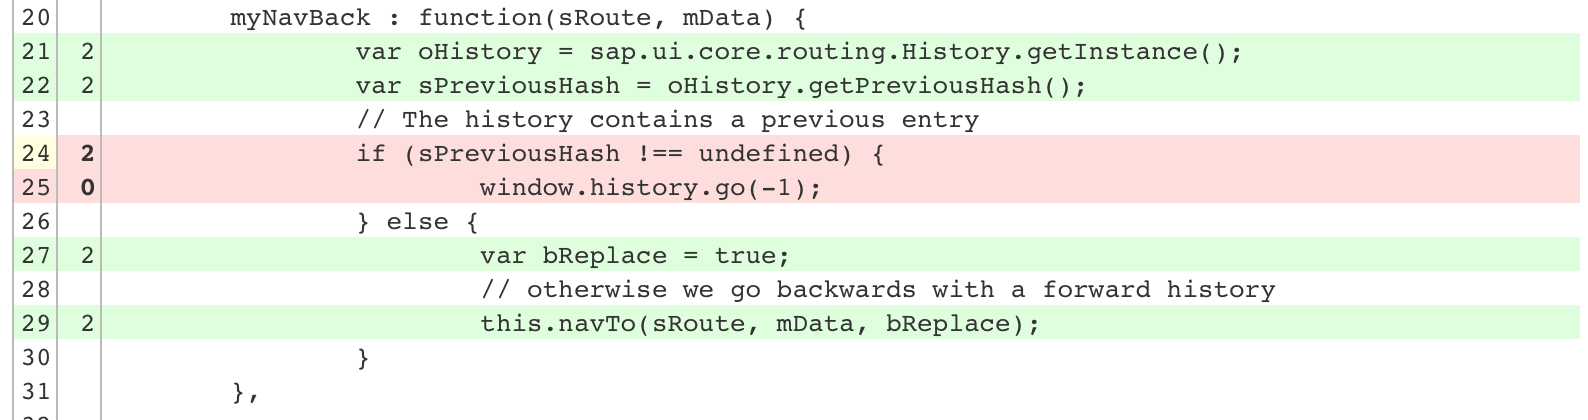
\includegraphics[width=1.25\textwidth]{CodeCoverage-Quellcode}
\caption[Zeilenabdeckung im Quellcode]{Zeilenabdeckung im Quellcode.}
\label{fig:CodeCoverage-Code}
\end{figure}

\subsubsection{HTML Publisher}
grunt-plato stellt die Ergebnisse der statischen Code-Analyse als HTML-Bericht zur Verfügung. Durch das Plugin wird in der Jenkins-Projektübersicht auf diesen Plato-Bericht verlinkt. Der Bericht zeigt Ergebnisse für das komplette Projekt oder auch für einzelne Dateien. In \autoref{fig:Platoresult} sieht man einen Report für die Datei Master3.controller.js.

\begin{figure}[h]
\centering
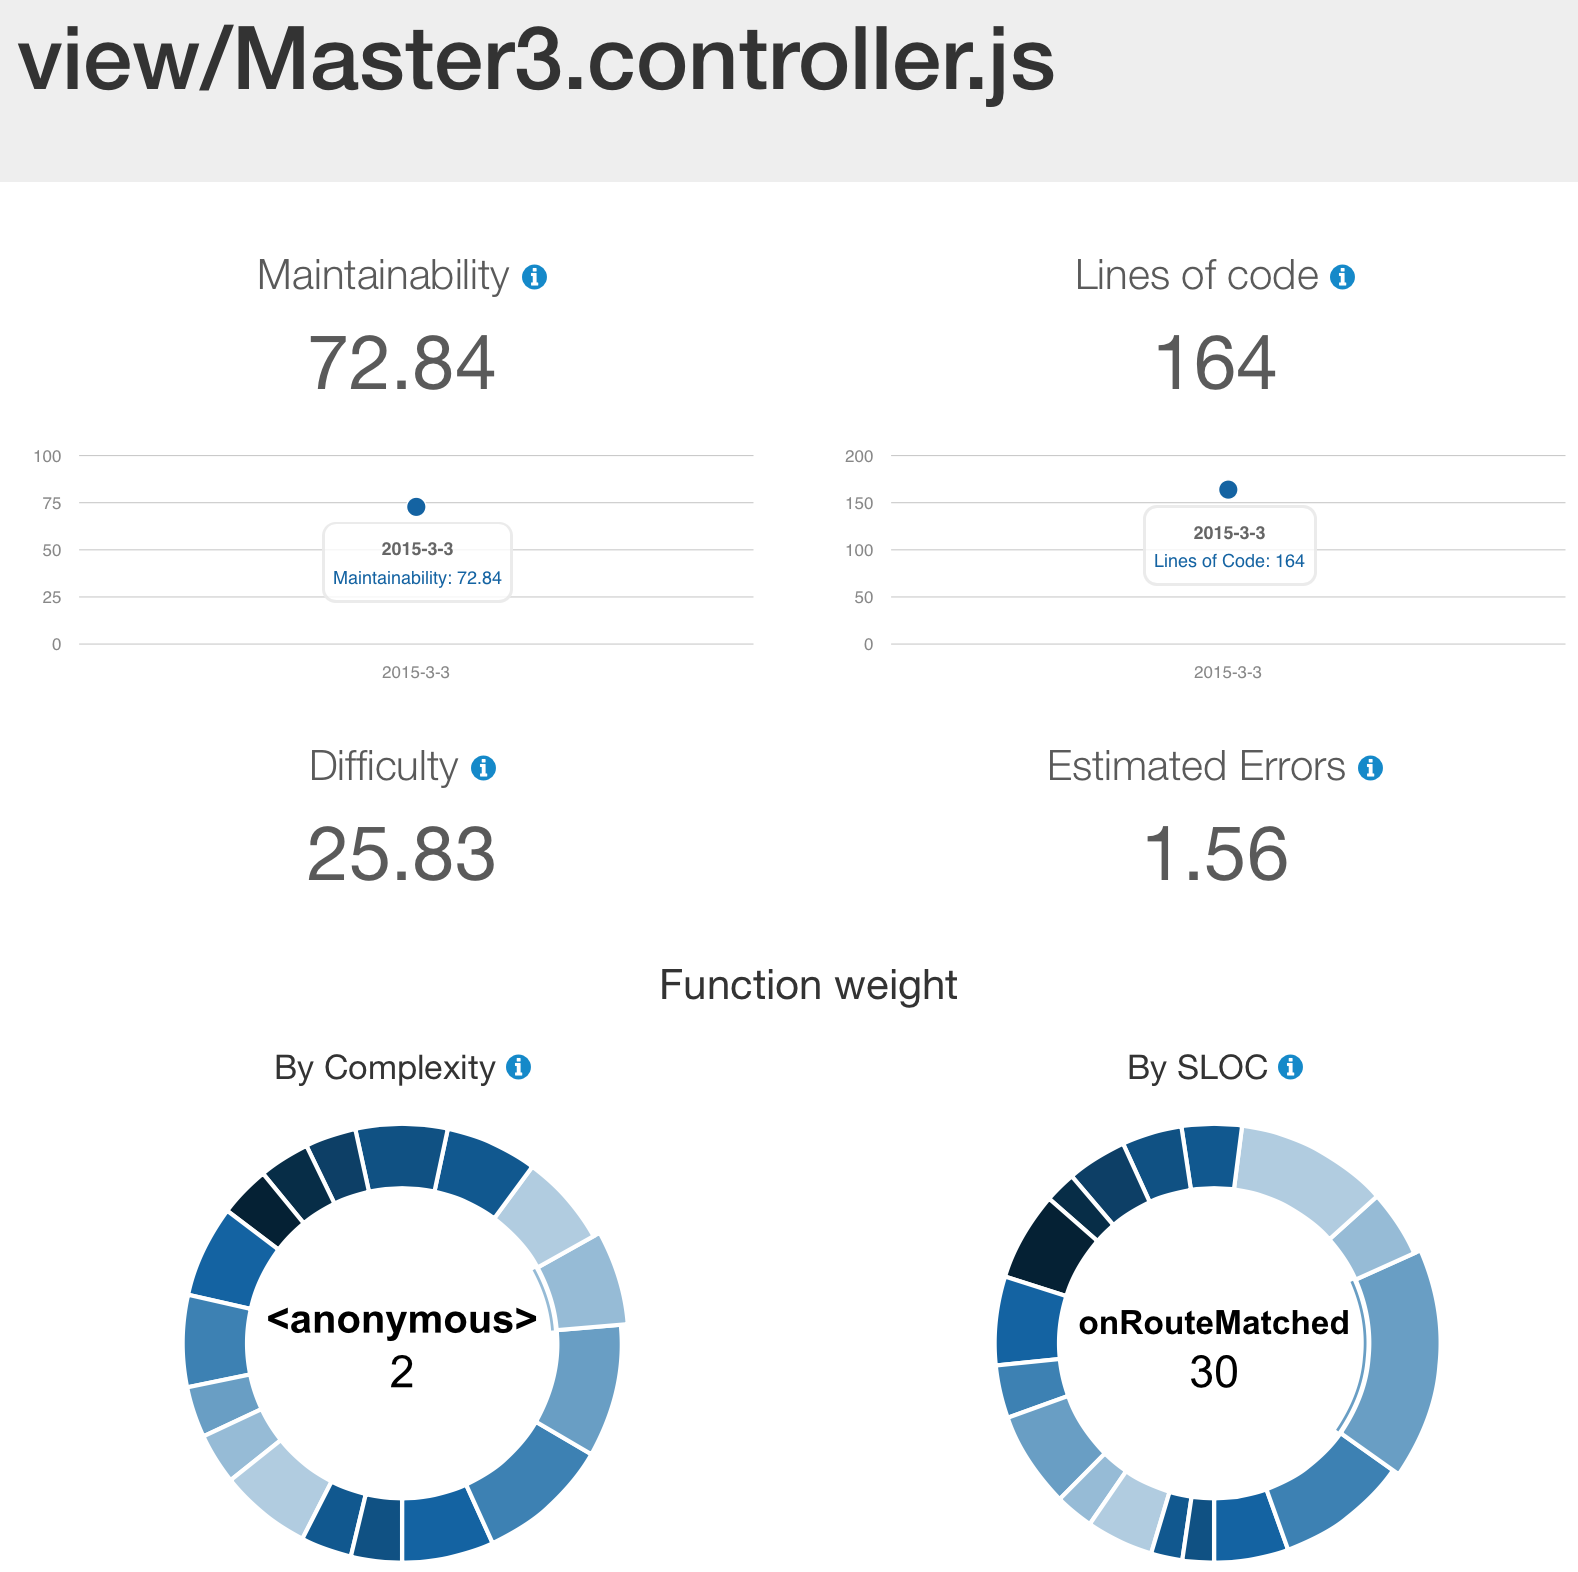
\includegraphics[width=.95\textwidth]{Plato2-JenkinsReport}
\caption[Plato-Bericht zu \emph{Master3.controller.js}]{Plato-Bericht zu \emph{Master3.controller.js}.}
\label{fig:Platoresult}
\end{figure}

\subsubsection{Timestamper}
Fügt der Konsolenausgabe von Jenkins einen Zeitstempel hinzu.

\subsubsection{Workspace Cleanup}
Ermöglicht das automatische Löschen des Arbeitsbereiches vor Ausführung des Builds. Da der komplette Prozess als Code abgebildet ist, wird permanent eine neue Build-Umgebung geschaffen.

% \begin{wrapfigure}[lines]{position}{breite}
\begin{wrapfigure}[4]{R}{2.5cm}
	\centering
	
\includegraphics{build_passing} 
	\caption[Build-Status]{Build-Status.}
	\label{fig:BuildStatus}
\end{wrapfigure}

\subsubsection{embeddable-build-status}
Erstellt ein Icon wie in \autoref{fig:BuildStatus} mit dem aktuellen Status des Builds zur Einbindung in Webseiten -- In unserem Fall in die GitHub Readme.

% Bugfix, Zeilennummern der Code-Listings sonst verschoben!
\begin{wrapfigure}[0]{l}{0cm}
\end{wrapfigure}

\newpage
\autsubsection{Zusammenfassung}{Azimi}
Die Testumgebung setzt sich aus drei großen Teilschritten zusammen. Diese sind die Build-Auslöser, der eigentliche Build-Prozess sowie die Post-Build-Operationen.

Build-Auslöser sind Ereignisse, die Jenkins dazu veranlassen einen neuen Build zu erstellen und alle Tests durchzuführen, die für dieses Projekt definiert wurden.
Dabei unterscheiden wir unter folgenden Build-Auslösern:
\begin{enumerate}
\item Der regelmäßige Build - jeden Tag um Mitternacht
\item Der Build bei Änderungen im GitHub - bei jedem Push
\item Der manuelle Start eines Buildvorganges
\end{enumerate}

Nach dem gemeldeten Ereignis durch den Auslöser startet Jenkins den Build. Zu Beginn jedes Builds wird der Arbeitsbereich gelöscht, um eine neue Build-Umgebung zu schaffen und die aktuelle Version des Quellcodes aus dem GitHub Repository herunterzuladen. Anschließend werden die benötigten Werkzeuge und Bibliotheken heruntergeladen und Grunt gestartet.

\SuperPar Im Build-Prozess werden schrittweise folgende Schritte ausgeführt:

\begin{enumerate}
\item Löschen des Arbeitsbereiches für einen sauberen Build
\item Code-Analyse durch ESLint und Plato
\item QUnit-Testausführung mit Karma inklusive Überprüfung der Zeilenabdeckung durch die QUnit bzw. OPA5-Tests
\item Kopieren der, für die App, notwendigen Dateien und Programmbibliotheken in den Target-Ordner
\item Komprimierung des JavaScript-Codes durch Uglify
\item Archivierung des Target-Ordners in eine ZIP-Datei
\item Hochladen der ZIP-Datei zu PhoneGap Build zum Kompilieren der Anwendung
\end{enumerate}

Zum Abschluss werden aus den Ergebnissen der verschiedenen Tests Berichte erzeugt und über die Jenkins-Oberfläche bereitgestellt. Die fertig kompilierte Anwendung lässt sich nun über PhoneGap Build auf den Geräten installieren. Die Dateistruktur des Projektes sieht nun so aus:

\begin{itemize}
	\item app/
	\item bower\_components/
	\item node\_modules/
	\item target/	
	\item test/
	\item test-reports/
	\item .eslintrc
	\item .gitignore
	\item bower.json
	\item config.xml
	\item Gruntfile.js
	\item karma.conf.js	
	\item package.json
\end{itemize}
\autsection{UI5-App}{Mattfeld}
\subsection{Auswahl der Entwicklungsumgebung}
\label{sec:auswahl_ide}

\subsubsection{Das bietet SAP}
Die von der SAP vorgeschlagene Universal-Entwicklungsumgebung ist Eclipse. Sie gehört \textit{noch} zur Firmenstrategie und wird mit einigen Plugins\footnote{\url{https://tools.hana.ondemand.com/}} einsatzbereit für die Entwicklung im SAP-Umfeld gemacht. Sie unterstützt unter anderem 
\begin{itemize}
	\item ABAP Development Tools for SAP NetWeaver
	\item SAP HANA Cloud Platform Tools
	\item Gateway (SAP Mobile Platform Tools)
	\item UI Development Toolkit for HTML5
\end{itemize}
Über die Transaktion \textit{/UI5/UI5\_REPOSITORY\_LOAD} werden UI5-Apps als \ac{BSP} auf einem SAP Web Application Server bereitgestellt. Das ist die Standard-Methode für Fiori-Apps. Die Transaktion ist remotefähig und wird per HTTP-Aufruf in eine CI-Toolchain eingebunden. Die gleiche Deploymentfunktion in Eclipse stellt der ABAP Repository Team Provider bereit.

Nicht zwingend notwendig, aber nützlich für die Backend-Entwicklung, ist der grafische OData Modeler aus den SAP Mobile Platform Tools, siehe \autoref{sec:OData-Modeler}. Er erleichtert Kommunikation und Abstimmung zwischen den Entwicklern. Die generierten Metadaten können sowohl im Gateway, als auch in SAPUI5 genutzt werden, ohne dass der eigentliche Service schon implementiert sein muss.

Das UI Development Toolkit for HTML5 enthält für die Frontend-Entwicklung:
\begin{itemize}
	\item App-Templates
	\item Test-Webserver
	\item Code-Vervollständigung
	\item XML-Syntaxprüfung
\end{itemize}
Ein schneller Einstieg in die UI5-Entwicklung ist mit diesen Tools möglich, sie sind jedoch keine Alleinstellungsmerkmale für Eclipse mit Plugin als \ac{IDE}. Sie sind auch in anderen Umgebungen verfügbar. Vielmehr sind die Templates für größere Projekte oder Nutzung als Fiori App durch fehlende Modularisierung sogar ungeeignet.

Noch schneller gelingt der Start mit der neuen SAP Web IDE\footnote{\url{http://scn.sap.com/docs/DOC-55465}}. Die Umgebung basiert auf Eclipse Orion und ist nach dem Login direkt startbereit. Dort sind modulare Templates für Fiori- und Hybrid-Apps verfügbar, die den aktuellen Best Practices folgen. Zu den weiteren Funktionen zählen:
\begin{itemize}
	\item Grafischer Layout-Editor 
	\item Live-Vorschau
	\item Code-Vervollständigung
	\item HANA Cloud Platform und ABAP-Repositories
	\item Mock-Daten-Support
\end{itemize}
Die ersten Erfahrungen mit der Web IDE sind vielversprechend: Die Anwendung reagiert schnell und implementiert außerdem anpassbare Code-Checks per ESLint und git-Support. Die Entwicklung schreitet schnell voran und soll auf lange Sicht Eclipse als UI5-IDE ablösen. 

Der Aufwand zur Entwicklung von Hybrid-Apps ist nicht verringert worden. Alle bekannten Build-Tools wie das Android SDK, Cordova, das Kapsel SDK u.\,a. müssen wie bisher lokal installiert und konfiguriert werden. Die Integration der Web IDE in externe Test- oder CI-Toolchains ist nicht möglich.

\subsubsection{Was benötigen wir?}
Wichtig sind möglichst wenig Kontextwechsel während der Entwicklung und damit eine hochintegrierte Entwicklungsumgebung. Das Werkzeug soll in den Hintergrund rücken und \ac{TDD} aktiv unterstützen. Wir wollen die gleiche Toolchain wie auf dem Integrationsserver nutzen.
Konkret benötigen wir:
\begin{itemize}
	\item Syntax-Hervorhebung der genutzten Sprache (JavaScript)
	\item Code-Vervollständigung der Frameworks (UI5)
	\item Integration von statischen Code-Analysen per ESlint
	\item QUnit-Testausführung per Karma
	\item Visualisierung der Code-Coverage
	\item Paketverwaltung per npm und Bower
	\item Grunt-Taskverwaltung
\end{itemize}
Eclipse beinhaltet im Auslieferungszustand nur wenig davon und die vorhandenen Funktionen wie Code-Vervollständigung in JavaScript-Projekten funktionieren nur selten. Manche der TDD-Funktionen ließen sich theoretisch per Plugin nachrüsten. Grunt als zentraler Task Runner aber \zB nicht. Da die vorhandene SAP-Integration allein Eclipse als IDE nicht rechtfertigt, wählen wir eine alternative IDE mit JavaScript- und TDD-Fokus.

\subsubsection{Lösung: WebStorm}
Gerade unter Web-Entwicklern genießt JetBrains WebStorm\footnote{\url{https://www.jetbrains.com/webstorm/}} einen hervorragenden Ruf: Die IDE ist speziell auf JavaScript-Projekte angepasst und bringt, neben zahlreichen Plugins, eine sinnvolle Vorkonfiguration mit. Schon aus früheren Projekten ist uns auch die Reaktionsfreude der zugrunde liegenden IntelliJ-Plattform bekannt. Wie können die bisher Eclipse-exklusiven Funktionen genutzt werden?

Die Syntax-Püfung von XML-Views ist über die entsprechenden XML-Definitionen (*.xsd) verfügbar. Diese sind Bestandteil des UI5 Development Toolkits for Eclipse, aber auch separat auf GitHub erhältlich\footnote{\url{https://github.com/jbmurray/UI5-WebStorm-Files}}. Das gleiche Repository enthält Bibliotheken, die sich für die UI5-Code-Vervollständigung in WebStorm nutzen lassen.
%\footnote{\url{http://scn.sap.com/community/developer-center/front-end/blog/2014/09/22/configuring-jetbrains-webstorm-for-ui5-development}}

Das ABAP Team Repository kann nicht integriert werden. Einchecken als \ac{BSP} aus WebStorm ist nur über den externen Aufruf einer Transaktion möglich. Für Fiori-Apps ist das verschmerzbar, da der CI-Server das finale Deployment übernimmt. Für hybride Apps spielt es ohnehin keine Rolle -- Installationspakete werden auf anderen Wegen verteilt, \zB über die App Stores oder eine \ac{MDM}-Lösung wie SAP Afaria.

\begin{figure}[h]
	\centering
	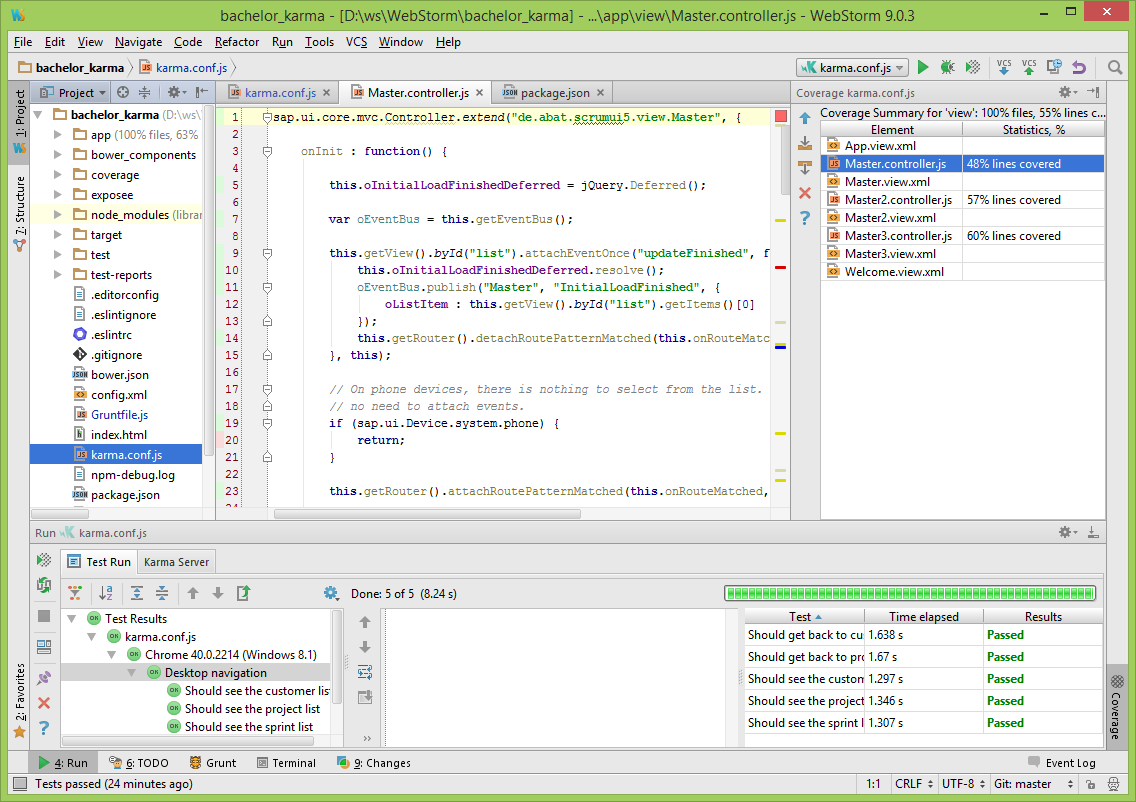
\includegraphics[width=1.25\textwidth]{WebStorm} 
	\caption[WebStorm mit TDD-Integration]{WebStorm mit TDD-Integration.}
	\label{fig:WebStorm}
\end{figure}

Webstorm integriert alle geforderten \ac{TDD}-Funktionen. \autoref{fig:WebStorm} zeigt die Ausführung von Karma-Tests in der \ac{IDE}. Test-Status und Code-Abdeckung werden direkt im Quellcode visualisiert. Grün markierte Zeilen wurden getestet, rote nicht. Um die testgetriebene Entwicklung in einer neuen WebStorm-Installation fortzusetzen sind folgende Schritte nötig:
\begin{enumerate}
	\item Klonen des Projekt-Repositories
	\item Installieren der Entwicklungs-Abhängigkeiten per \emph{npm install}
	\item Installieren der Frontend-Abhängigkeiten per \emph{bower install}
\end{enumerate}
Die Test-Konfiguration muss nicht angepasst werden -- WebStorm nutzt die, bereits als Code vorliegende, CI-Toolchain mit ihren Grunt-Tasks automatisch. Die Toolchain wird nicht nur abgespielt, sondern kann auch mit IDE-Unterstützung bearbeitet werden. WebStorm hat eigene Paketverwaltungen für Node.js und Bower, die sich entsprechend nutzen lassen.

Auch viele der weiteren Konfigurationsdateien werden automatisch erkannt. Die statische Code-Analyse erfolgt parallel mithilfe der eigenen ESLint-Regeln. Automatische Code-Formatierung orientiert sich an der IDE-übergreifenden \emph{.editorconfig}. Selbst die \emph{.gitignore}-Konfiguration findet bei der Nachverfolgung lokaler Änderungen Verwendung.

Insgesamt wird die Entwicklung durch WebStorm aktiv unterstützt. Alles was automatisiert werden kann, wird es auch. Die Benutzererfahrung ist deutlich besser als unter Eclipse, wo vieles nur langsam oder gar nicht funktioniert. Gegenüber der SAP Web IDE ist die Integration und Weiterentwicklungsmöglichkeit der CI-Toolchain sehr gelungen.


\subsection{UI5-App}
Abbildung \ref{fig:app_main_screen} zeigt den Hauptbildschirm der entwickelten UI5-Scrum-App. Sie ist nach dem typischen Master-Detail-Konzept gestaltet: In der linken Master-View wird erst ein Kunde ausgewählt, dann ein Projekt und Sprint. Anschließend zeigt die große Detail-View rechts die entsprechenden Sprint-Daten. Die Ansicht ist responsive, wird bei kleineren Bildschirmen also automatisch angepasst.

\begin{figure}
	\centering
	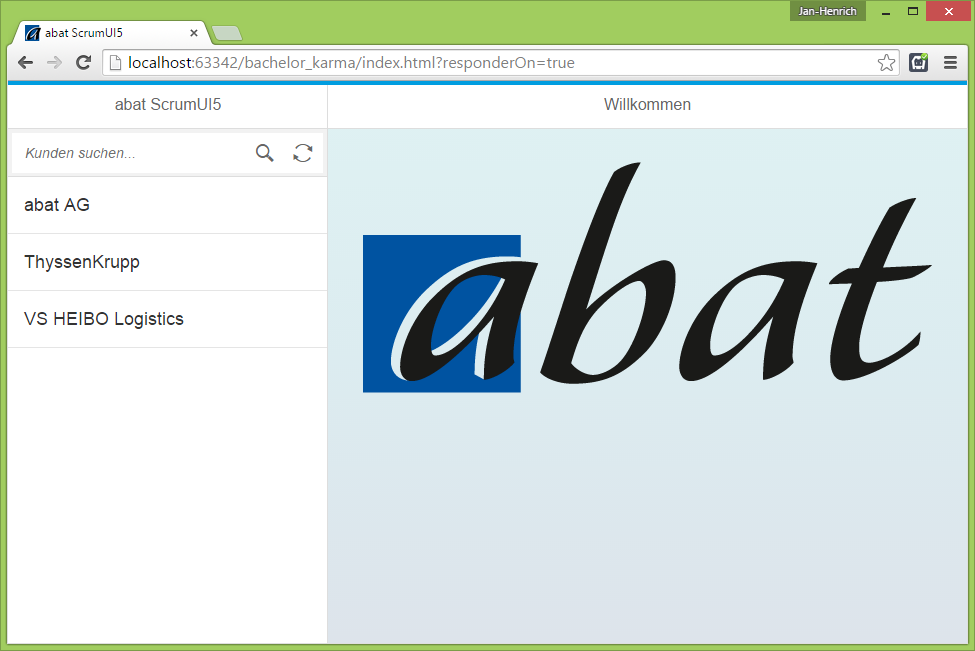
\includegraphics[width=0.95\textwidth]{app_main_screen} 
	\caption[UI5-App -- Hauptbildschirm]{UI5-App -- Hauptbildschirm mit Mock-Daten.}
	\label{fig:app_main_screen}
\end{figure}

Intern entspricht die App dem Model-View-Controller-Prinzip. Daraus ergibt sich folgende (gekürzte) Dateistruktur, die den aktuellen Best Practices entspricht:
\begin{itemize}
	\item app/
	\begin{itemize}
		\item i18n/
		\begin{itemize}
			\item messageBundle.properties
			\item messageBundle\_de\_DE.properties
		\end{itemize}		
%		\item img/
%		\begin{itemize}
%			\item background\_logo.png
%			\item favicon.ico
%		\end{itemize}
		\item view/
		\begin{itemize}
			\item Master.view.xml
			\item Master.controller.js
		\end{itemize}
		\item Component.js
		\item index.html
		\item MyRouter.js
	\end{itemize}
\end{itemize}

\subsubsection{Kapselung}
Als Startpunkt dient die \textit{index.html}, sie ermöglicht die Ausführung der App im Browser. Metatags geben dem Browser Hinweise zur korrekten Darstellung. Danach findet nur noch das Bootstrapping, also Laden, der UI5-Bibliotheken statt. Anschließend wird die App in einem Shell-Container gestartet.

Die eigentliche App ist unabhängig von einer HTML-Datei in der \textit{Component.js} definiert. Durch diese Kapselung ist die App portabel. Eine weitere Ausführungsumgebung ist \zB das Fiori Launchpad. In der Komponente sind allgemeine Informationen wie App-Name und Version gespeichert. Ebenso festgelegt ist die erste aufzurufende View.

\subsubsection{Routing}
Daneben enthält \textit{Component.js} die Routen-Konfiguration. Das Routing-Konzept ist Teil der Kapselung, da die Navigation innerhalb der App über einen eigenen Router (\textit{MyRouter.js}) stattfindet. In Ausführungsumgebungen mit mehreren UI5-Apps werden Konflikte vermieden.

Weiterer Vorteil: Über bestimmte URLs ist immer der gleiche App-Zustand erreichbar. Wie von anderen Webanwendungen gewohnt, kann über den Parameter \textit{/Kunden(Kunde='ABAT')/Projekte} immer die Projektübersicht des Kunden, in diesem Fall abat, aufgerufen werden. Die entsprechende Seite lässt sich bequem als Lesezeichen speichern.

\subsubsection{Internationalisierung}
Statische Texte sind in Resource Bundles wie \textit{messageBundle\_de.properties} definiert. Sie enthalten Schlüssel/Wert-Paare mit der entsprechenden Übersetzung in einer bestimmten Sprache und Landeskennung. Englische Standardtexte sind grundsätzlich in \textit{messageBundle.properties} gespeichert. 

In einer XML-View wird statischer Text wie \textit{i18n>masterTitle} automatisch mit dem Pendant aus dem i18n-Model ersetzt. Die aktuelle Sprache wird \zB aus dem Browser, dem Betriebssystem oder einem URL-Parameter bestimmt. UI5 sucht automatisch das passende Resource Bundle.

\subsubsection{OData}
Die Adresse des OData-Services ist ebenfalls in der \textit{Component.js} festgelegt. Während der Initialisierung werden die Metadaten geladen und als globales App-Model festgelegt. 
Anschließend werden die Elemente einer Liste \zB über \textit{items='{/Kunden}'} entsprechend der Einträge im Pfad des OData-Services angezeigt. 
Bei einem Klick auf den Kunden, wird dieser als aktueller \textit{BindingContext} gespeichert. Die Elemente der nachfolgenden Liste werden dann unter \textit{{gespeicherterKunde}/Projekte} gesucht. An dieser Stelle greifen UI5 und die Navigationseigenschaften des OData-Services ineinander.

\subsection{Akzeptanztests mit OPA5}
OPA5 basiert auf QUnit und ermöglicht Akzeptanztests für UI5-Apps. Es erleichtert die Test-Programmierung durch spezielle Selektoren für UI5-Controls und die Verwaltung von Asynchronität.

Analog zu den Testfall-Szenarien im \autoref{sec:tests} werden Tests per \textit{Given/When/Then} definiert. Die Formulierung aus den Testfällen lässt sich fast direkt in Code umsetzen, siehe Listing \ref{lst:opa5}. Voraussetzung hierfür ist die vorherige Definition zahlreicher eigener \textit{Actions} und \textit{Assertions}. 

Ein Beispiel ist die Assertion \textit{iShouldSeeTheCustomerList()}. Diese wird aus \textit{NavigationAssertions.js} nachgeladen und dem Framework über \textit{extendConfig()} bekannt gemacht. Innerhalb der nachgeladenen Datei ruft sie generellere Funktionen wie \textit{iClickOnAListItem(listName)} auf. Hierüber ist eine grundsätzliche Modularisierung der Tests möglich.

Nur für bestimmte Views nützliche Testfunktionen werden diesen über PageObjects zugeteilt und automatisch mitgeladen. Dies erleichtert die Strukturierung. Trotzdem wird das Testprojekt bei größerem Umfang schnell unübersichtlich. Die meisten Funktionen müssen selbst erstellt werden. Ein grafischer Editor, wie \zB Jubula ihn mitbringt, wäre von großem Vorteil.

Die OPA5-Tests können über eine HTML-Datei gestartet werden. Diese dient nur als Container, analog zum Start der normalen App-Komponente. Dort werden sie wie klassische QUnit-Tests in einem iFrame ausgeführt. In unserer Toolchain genügt eine JavaScript-Datei wie Listing \ref{lst:opa5}, die von Karma ausgeführt wird.

Die Implementierung des Mockservers ist bereits in \autoref{sec:karma} beschrieben. Er wird über den URL-Parameter \textit{?responderOn=true} aktiviert. Der Test läuft jetzt auch ohne Verbindung zum Backend.
%Die gekürzte Verzeichnisstruktur der Tests:
%\begin{itemize}
%	\item test/
%	 \begin{itemize}
%		\item actions/
%		\item arrangements/
%		\item assertions/
%		\item Navigations.js
%%		\item opaTests.qunit.html
%	\end{itemize}
%\end{itemize}

\begin{listing}[H]
	\inputminted[tabsize=2]{js}{src/opa5.js}
	\caption{OPA5-Test-Szenario 1}
	\label{lst:opa5}
\end{listing}
